%======================================================================
% University of Waterloo Thesis Template for LaTeX
% Last Updated August 2023
% by IST Client Services,
% University of Waterloo, 200 University Ave. W., Waterloo, Ontario, Canada
% FOR ASSISTANCE, please send mail to ist-helpdesk@uwaterloo.ca

% DISCLAIMER
% To the best of our knowledge, this template satisfies the current uWaterloo thesis requirements.
% However, it is your responsibility to assure that you have met all requirements of the University and your particular department.

% Many thanks for the feedback from many graduates who assisted the development of this template.
% Also note that there are explanatory comments and tips throughout this template.
%======================================================================
% Some important notes on using this template and making it your own...

% The University of Waterloo has required electronic thesis submission since October 2006.
% See the uWaterloo thesis regulations at
% https://uwaterloo.ca/graduate-studies/thesis.
% This thesis template is geared towards generating a PDF version optimized for viewing on an electronic display, including hyperlinks within the PDF.

% DON'T FORGET TO ADD YOUR OWN NAME AND TITLE in the "hyperref" package configuration below.
% Search for: PDFTITLE, PDFAUTHOR, PDFSUBJECT, and PDFKEYWORDS.
% THIS INFORMATION GETS EMBEDDED IN THE FINAL PDF DOCUMENT.
% You can view the information if you view properties of the PDF document.

% Many faculties/departments also require one or more printed copies.
% This template attempts to satisfy both types of output.
% See additional notes below.
% It is based on the standard "book" document class which provides all necessary sectioning structures and allows multi-part theses.

% If you are using this template in Overleaf (cloud-based collaboration service), then it is automatically processed and previewed for you as you edit.

% For people who prefer to install their own LaTeX distributions on their own computers, and process the source files manually, the following notes provide the sequence of tasks:

% E.g. to process a thesis called "mythesis.tex" based on this template, run:

% pdflatex mythesis	-- first pass of the pdflatex processor
% bibtex mythesis	-- generates bibliography from .bib data file(s)
% makeindex         -- should be run only if an index is used
% pdflatex mythesis	-- fixes numbering in cross-references, bibliographic references, glossaries, index, etc.
% pdflatex mythesis	-- it takes a couple of passes to completely process all cross-references

% If you use the recommended LaTeX editor, Texmaker, you would open the mythesis.tex file, then click the PDFLaTeX button. Then run BibTeX (under the Tools menu).
% Then click the PDFLaTeX button two more times.
% If you have an index as well,you'll need to run MakeIndex from the Tools menu as well, before running pdflatex
% the last two times.

% N.B. The "pdftex" program allows graphics in the following formats to be included with the "\includegraphics" command: PNG, PDF, JPEG, TIFF
% Tip: Generate your figures and photos in the size you want them to appear in your thesis, rather than scaling them with \includegraphics options.
% Tip: Any drawings you do should be in scalable vector graphic formats: SVG, PNG, WMF, EPS and then converted to PNG or PDF, so they are scalable in the final PDF as well.
% Tip: Photographs should be cropped and compressed so as not to be too large.

% To create a PDF output that is optimized for double-sided printing:
% 1) comment-out the \documentclass statement in the preamble below, and un-comment the second \documentclass line.
% 2) change the value assigned below to the boolean variable "PrintVersion" from " false" to "true".

%======================================================================
%   D O C U M E N T   P R E A M B L E
% Specify the document class, default style attributes, and page dimensions, etc.
% For hyperlinked PDF, suitable for viewing on a computer, use this:
\documentclass[letterpaper,12pt,titlepage,oneside,final]{book}

% For PDF, suitable for double-sided printing, change the PrintVersion variable below to "true" and use this \documentclass line instead of the one above:
%\documentclass[letterpaper,12pt,titlepage,openright,twoside,final]{book}

% Some LaTeX commands I define for my own nomenclature.
% If you have to, it's easier to make changes to nomenclature once here than in a million places throughout your thesis!
\newcommand{\package}[1]{\textbf{#1}} % package names in bold text
\newcommand{\cmmd}[1]{\textbackslash\texttt{#1}} % command name in tt font
\newcommand{\href}[1]{#1} % does nothing, but defines the command so the print-optimized version will ignore \href tags (redefined by hyperref pkg).
%\newcommand{\texorpdfstring}[2]{#1} % does nothing, but defines the command
% Anything defined here may be redefined by packages added below...

% This package allows if-then-else control structures.
\usepackage{ifthen}
\newboolean{PrintVersion}
\setboolean{PrintVersion}{false}
% CHANGE THIS VALUE TO "true" as necessary, to improve printed results for hard copies by overriding some options of the hyperref package, called below.

% Added for writing code
\usepackage{listings}
\usepackage{xcolor}
\usepackage{tikz}
\usetikzlibrary{arrows.meta, positioning}
\usepackage{amsmath, amssymb}
\usepackage{seqsplit}

\lstset{
  basicstyle=\ttfamily,
  keywordstyle=\color{blue},
  commentstyle=\color{gray},
  stringstyle=\color{red},
  numbers=left,
  numberstyle=\tiny\color{gray},
  stepnumber=1,
  numbersep=5pt,
  tabsize=4,
  showspaces=false,
  showstringspaces=false,
  frame=single,
  breaklines=true
}

\usepackage{titlesec}

% For making result boxes
\usepackage[most]{tcolorbox}

\newtcolorbox{findingbox}[1][]{
  colback=gray!10!white,
  colframe=gray!50!black,
  #1
}

% For making todos
\usepackage{todonotes}

% For making tables
\usepackage{tabularray}
\usepackage{tabularx}
\usepackage{booktabs}
\usepackage{ragged2e}
\usepackage{makecell} % For automatic word breakin
\usepackage[margin=1in]{geometry}
\usepackage{longtable}
\usepackage{array}         % For column types
\usepackage{calc}
\usepackage{lipsum}



% Define custom column type with hanging indent
\newcolumntype{H}[1]{>{\hangindent=1em\hangafter=1\RaggedRight\arraybackslash}p{#1}}

%\usepackage{nomencl} % For a nomenclature (optional; available from ctan.org)
\usepackage{amsmath,amssymb,amstext} % Lots of math symbols and environments
% \usepackage[pdftex]{graphicx} % For including graphics N.B. pdftex graphics driver

% Hyperlinks make it very easy to navigate an electronic document.
% In addition, this is where you should specify the thesis title and author as they appear in the properties of the PDF document.
% Use the "hyperref" package
% N.B. HYPERREF MUST BE THE LAST PACKAGE LOADED; ADD ADDITIONAL PKGS ABOVE
\usepackage[pdftex,pagebackref=false]{hyperref} % with basic options
%\usepackage[pdftex,pagebackref=true]{hyperref}
		% N.B. pagebackref=true provides links back from the References to the body text. This can cause trouble for printing.
\hypersetup{
    plainpages=false,       % needed if Roman numbers in frontpages
    unicode=false,          % non-Latin characters in Acrobat’s bookmarks
    pdftoolbar=true,        % show Acrobat’s toolbar?
    pdfmenubar=true,        % show Acrobat’s menu?
    pdffitwindow=false,     % window fit to page when opened
    pdfstartview={FitH},    % fits the width of the page to the window
%    pdftitle={uWaterloo\ LaTeX\ Thesis\ Template},    % title: CHANGE THIS TEXT!
%    pdfauthor={Author},    % author: CHANGE THIS TEXT! and uncomment this line
%    pdfsubject={Subject},  % subject: CHANGE THIS TEXT! and uncomment this line
%    pdfkeywords={keyword1} {key2} {key3}, % list of keywords, and uncomment this line if desired
    pdfnewwindow=true,      % links in new window
    colorlinks=true,        % false: boxed links; true: colored links
    linkcolor=blue,         % color of internal links
    citecolor=green,        % color of links to bibliography
    filecolor=magenta,      % color of file links
    urlcolor=cyan           % color of external links
}
\ifthenelse{\boolean{PrintVersion}}{   % for improved print quality, change some hyperref options
\hypersetup{	% override some previously defined hyperref options
%    colorlinks,%
    citecolor=black,%
    filecolor=black,%
    linkcolor=black,%
    urlcolor=black}
}{} % end of ifthenelse (no else)

\usepackage[automake,toc,abbreviations]{glossaries-extra} % Exception to the rule of hyperref being the last add-on package
% If glossaries-extra is not in your LaTeX distribution, get it from CTAN (http://ctan.org/pkg/glossaries-extra),
% although it's supposed to be in both the TeX Live and MikTeX distributions. There are also documentation and
% installation instructions there.

% Setting up the page margins...
% uWaterloo thesis requirements specify a minimum of 1 inch (72pt) margin at the
% top, bottom, and outside page edges and a 1.125 in. (81pt) gutter margin (on binding side).
% While this is not an issue for electronic viewing, a PDF may be printed, and so we have the same page layout for both printed and electronic versions, we leave the gutter margin in.
% Set margins to minimum permitted by uWaterloo thesis regulations:
\setlength{\marginparwidth}{0pt} % width of margin notes
% N.B. If margin notes are used, you must adjust \textwidth, \marginparwidth
% and \marginparsep so that the space left between the margin notes and page
% edge is less than 15 mm (0.6 in.)
\setlength{\marginparsep}{0pt} % width of space between body text and margin notes
\setlength{\evensidemargin}{0.125in} % Adds 1/8 in. to binding side of all
% even-numbered pages when the "twoside" printing option is selected
\setlength{\oddsidemargin}{0.125in} % Adds 1/8 in. to the left of all pages when "oneside" printing is selected, and to the left of all odd-numbered pages when "twoside" printing is selected
\setlength{\textwidth}{6.375in} % assuming US letter paper (8.5 in. x 11 in.) and side margins as above
\raggedbottom

% The following statement specifies the amount of space between paragraphs. Other reasonable specifications are \bigskipamount and \smallskipamount.
\setlength{\parskip}{\medskipamount}

% The following statement controls the line spacing.
% The default spacing corresponds to good typographic conventions and only slight changes (e.g., perhaps "1.2"), if any, should be made.
\renewcommand{\baselinestretch}{1} % this is the default line space setting

% By default, each chapter will start on a recto (right-hand side) page.
% We also force each section of the front pages to start on a recto page by inserting \cleardoublepage commands.
% In many cases, this will require that the verso (left-hand) page be blank, and while it should be counted, a page number should not be printed.
% The following statements ensure a page number is not printed on an otherwise blank verso page.
\let\origdoublepage\cleardoublepage
\newcommand{\clearemptydoublepage}{%
  \clearpage{\pagestyle{empty}\origdoublepage}}
\let\cleardoublepage\clearemptydoublepage

% Define Glossary terms (This is properly done here, in the preamble and could also be \input{} from a separate file...)
% Main glossary entries -- definitions of relevant terminology
\newglossaryentry{computer}
{
name=computer,
description={A programmable machine that receives input data,
               stores and manipulates the data, and provides
               formatted output}
}

% Nomenclature glossary entries -- New definitions, or unusual terminology
\newglossary*{nomenclature}{Nomenclature}
\newglossaryentry{dingledorf}
{
type=nomenclature,
name=dingledorf,
description={A person of supposed average intelligence who makes incredibly brainless misjudgments}
}

% List of Abbreviations (abbreviations type is built in to the glossaries-extra package)
\newabbreviation{api}{API}{Application Programming Interface}
\newabbreviation{bbc}{BBC}{behavioural breaking change}

% List of Symbols
\newglossary*{symbols}{List of Symbols}
\newglossaryentry{rvec}
{
name={$\mathbf{v}$},
sort={label},
type=symbols,
description={Random vector: a location in n-dimensional Cartesian space, where each dimensional component is determined by a random process}
}
\makeglossaries

%======================================================================
%   L O G I C A L    D O C U M E N T
% The logical document contains the main content of your thesis.
% Being a large document, it is a good idea to divide your thesis into several files, each one containing one chapter or other significant chunk of content, so you can easily shuffle things around later if desired.
%======================================================================
\begin{document}

%----------------------------------------------------------------------
% FRONT MATERIAL
% title page, examining committee membership (for PhD Thesis only), declaration, borrowers' page, abstract, acknowledgements,
% dedication, table of contents, list of tables, list of figures, nomenclature, etc.
%----------------------------------------------------------------------
% T I T L E   P A G E
% -------------------
% Last updated August 24, 2023, by IST-Client Services
% The title page is counted as page `i' but we need to suppress the
% page number. Also, we don't want any headers or footers.
\pagestyle{empty}
\pagenumbering{roman}

% The contents of the title page are specified in the "titlepage"
% environment.
\begin{titlepage}
        \begin{center}
        \vspace*{1.0cm}

        \Huge
        {\bf Detecting Unchecked Exception-Related Behavioural Breaking Changes with UnCheckGuard }

        \vspace*{1.0cm}

        \normalsize
        by \\

        \vspace*{1.0cm}

        \Large
        Vinayak Sharma \\

        \vspace*{3.0cm}

        \normalsize
        A thesis \\
        presented to the University of Waterloo \\ 
        in fulfillment of the \\
        thesis requirement for the degree of \\
        Master of Applied Science \\
        in \\
        Electrical and Computer Engineering \\

        \vspace*{1.0cm}

        Waterloo, Ontario, Canada, 2025 \\

        \vspace*{1.0cm}

        \copyright\ Vinayak Sharma 2025 \\
        \end{center}
\end{titlepage}

% The rest of the front pages should contain no headers and be numbered using Roman numerals starting with `ii'
\pagestyle{plain}
\setcounter{page}{2}

\cleardoublepage % Ends the current page and causes all figures and tables that have so far appeared in the input to be printed.
% In a two-sided printing style, it also makes the next page a right-hand (odd-numbered) page, producing a blank page if necessary.
\phantomsection    % allows hyperref to link to the correct page
 

% D E C L A R A T I O N   P A G E
% -------------------------------
  % The following is a sample Declaration Page as provided by the GSPA
  % December 13th, 2006.  It is designed for an electronic thesis.
 \addcontentsline{toc}{chapter}{Author's Declaration}
 \begin{center}\textbf{Author's Declaration}\end{center}

 % Author's Declaration Option ONE - line 118:  
 \noindent
This thesis consists of material all of which I authored or co-authored: see Statement of
Contributions included in the thesis. This is a true copy of the thesis, including any required final revisions, as accepted by my examiners.
  % Author's Declaration Option TWO - line 121. Updated August 21st, 2023. Use the following declaration text if appropriate by removing the percent character and space at the beginning of line 121, and add a percent symbol and space at line 118 to change Author's Declaration Option ONE to a remark that is not printed.
 \noindent  
% This thesis consists of material all of which I authored or co-authored: see Statement of Contributions included in the thesis. This is a true copy of the thesis, including any required final revisions, as accepted by my examiners.
  \bigskip
  
  \noindent
I understand that my thesis may be made electronically available to the public.

\cleardoublepage
\phantomsection    % allows hyperref to link to the correct page

% S T A T E M E N T  O F  C O N T R I B U T I O N S
% -------------------------------
  % The following is a sample Declaration Page as provided by the GSPA
  % December 13th, 2006.  It is designed for an electronic thesis.
 \addcontentsline{toc}{chapter}{Statement of Contributions}
 \begin{center}\textbf{Statement of Contributions}\end{center}

This thesis primarily comprises chapters derived from our research paper which has been
submitted at SCAM 2025, incorporating wording changes, stylistic updates, and other
modifications.

Added to the original work are the following:

\begin{itemize}
  \item Adding information about software libraries and overview of the thesis in Chapter~\ref{intro}.
  \item Addition of Chapter~\ref{background} for explaining the core concepts related to the thesis.
  \item Further elaboration on the motivating example in Chapter~\ref{example}, addition of figures for explaining the call mades withing the library.
\end{itemize}

\cleardoublepage
\phantomsection    % allows hyperref to link to the correct page

% A B S T R A C T
% ---------------
\addcontentsline{toc}{chapter}{Abstract}
\begin{center}\textbf{Abstract}\end{center}

      The ubiquitous use of third-party libraries in software development has enabled developers to quickly add
      new functionality to their client software. Unfortunately, library usage also carries a cost in
      terms of software maintenance: library upgrades may include breaking changes, in which client expectations
      about library behaviour are no longer met in new library versions. Behavioural breaking
      changes can be particularly insidious, and in their full generality, could require sophisticated program
      analysis techniques to (approximately) detect.

      In this work, we present our UnCheckGuard tool, which detects a class of behavioural breaking changes---those
      related to exceptions thrown by Java libraries. UnCheckGuard analyzes both sides of the library/client
      duet. On the library side, UnCheckGuard creates a list of new exceptions that may be thrown by methods
      in a library's public API, including by its transitive callees. On the client side, UnCheckGuard identifies
      client methods that call library methods with new exceptions. To reduce false positives, UnCheckGuard
      additionally filters out new exceptions that cannot be triggered by particular clients, using taint analysis. It therefore can be
      used by client developers as a tool to screen library updates for relevant incompatibilities.

      We have evaluated UnCheckGuard on 69 libraries and 99 library-client pairs drawn from the DUETS collection
      and found 8 libraries with newly-added exceptions, as well as 49 callsites to library methods which,
      when upgraded to the latest version, may introduce
      a behavioural breaking change in the client due to a newly added unchecked exception. These findings
      highlight the practical value of UnCheckGuard in identifying exception-related incompatibilities
      introduced by library upgrades.

\cleardoublepage
\phantomsection    % allows hyperref to link to the correct page

% A C K N O W L E D G E M E N T S
% -------------------------------
\addcontentsline{toc}{chapter}{Acknowledgements}
\begin{center}\textbf{Acknowledgements}\end{center}

First and foremost, I would like to thank Dr. Patrik Lam for his unwavering support throughout every stage of my master's journey. His constant positivity and encouragement toward excellence made it possible for me to work on such an interesting topic. From narrowing down the research focus to perfecting the tool, he has guided me at every step of the research process. His mentorship has not only shaped the direction of my thesis but has also played a significant role in my growth as a researcher and academic.

I would also like to thank my parents and my sister for their continuous support. As professors, my parents have always inspired me to strive for academic excellence and have been a constant source of motivation throughout my life. My sister, in particular, has provided me with valuable advice on how to improve academically, which has been instrumental during this journey.

I am also grateful to the friends and individuals I have met along the way, whose support and encouragement have contributed to both my personal and academic well-being during this time.

Lastly, I would like to thank Dr. Weiyi Shang and Dr. Derek Rayside for their time and thoughtful feedback in reviewing my thesis.
\cleardoublepage
\phantomsection    % allows hyperref to link to the correct page


% D E D I C A T I O N
% -------------------------------
\addcontentsline{toc}{chapter}{Dedication}
\begin{center}\textbf{Dedication}\end{center}
This thesis is dedicated to my family.
\cleardoublepage
\phantomsection    % allows hyperref to link to the correct page



% T A B L E   O F   C O N T E N T S
% ---------------------------------
\renewcommand\contentsname{Table of Contents}
\tableofcontents
\cleardoublepage
\phantomsection    % allows hyperref to link to the correct page

% L I S T   O F   F I G U R E S
% -----------------------------
\addcontentsline{toc}{chapter}{List of Figures}
\listoffigures
\cleardoublepage
\phantomsection		% allows hyperref to link to the correct page

% L I S T   O F   T A B L E S
% ---------------------------
\addcontentsline{toc}{chapter}{List of Tables}
\listoftables
\cleardoublepage
\phantomsection		% allows hyperref to link to the correct page

% L I S T   O F   A B B R E V I A T I O N S
% ---------------------------
\renewcommand*{\abbreviationsname}{List of Abbreviations}
\printglossary[type=abbreviations]
\cleardoublepage
\phantomsection		% allows hyperref to link to the correct page

% L I S T   O F   S Y M B O L S
% ---------------------------
\printglossary[type=symbols]
\cleardoublepage
\phantomsection		% allows hyperref to link to the correct page


% Change page numbering back to Arabic numerals
\pagenumbering{arabic}



%----------------------------------------------------------------------
% MAIN BODY
% We suggest using a separate file for each chapter of your thesis.
% Start each chapter file with the \chapter command.
% Only use \documentclass or \begin{document} and \end{document} commands in this master document.
% Tip: Putting each sentence on a new line is a way to simplify later editing.
%----------------------------------------------------------------------
%======================================================================
\chapter{Introduction}\label{intro}
%======================================================================
% look for citations about library usage
Software libraries are mainly collections of code components designed to be reused
across projects at different levels, they help developers save time and effort by
eliminating the need to rewrite code, and their functionalities can be directly integrated
into software applications~\cite{Sawant2015APIUsage}. In the recent decades, the use of software libraries is
becoming more and more prominent as software libraries integration in the programs
allows the developers to develop the software more effectively~\cite{Cybulski2007requirements}. However, sometime
the developed software are required to be integrated with the updated versions of
libraries and their components, this allows the developers to upgrade and reuse the
software.

Software libraries are developed, maintained and upgraded by a range of contributors
that includes: (i) Individual developers, (ii) Open-source communities, (iii) Companies
(such as Google, Facebook, and Microsoft) and (iv) Academic and Research
institutions~\cite{Lakhani2000OSS}. The role of these contributors is to create libraries to meet specific needs
and their refinement over the period of time~\cite{Decan2018npm}. Others focus on managing community
contributions, maintaining code quality, and integrating updates. These roles ensure that
libraries remain reliable and up to date.

The dependence on software libraries has increased over time because of the increase in open source software (OSS) movement and the huge increase in software libraries on repository ecosystems such as npm for JavaScript, PyPI for Python, MAVEN for Java, and CRAN for R. Therefore, software development has become a highly modular activity and has a huge reliance on third-party libraries~\cite{decan2019empirical, kalliamvakou2014promises, zerouali2019formal, cox2019surviving}. However, libraries developed by others are also updated by others, on schedules that are not controlled by the client developers.

% Especially when one is developing software that is exposed to the Internet, one
% has a responsibility to incorporate security updates for the
% libraries that one is using as a client~\cite{wu23:_under_threat_upstr_vulner_downs}, or else risk vulnerabilities
% being exposed in one's software~\cite{haryono22:_autom_ident_librar_vulner_data,zhan21:_atvhun,alfadel23:_empir_python}. 
% The obligation to update libraries is a form of technical debt that accrues automatically with the passage of time.

When a client develops software exposed to the internet, they become responsible for ensuring that the application integrates security updates for all utilized software libraries~\cite{wu23:_under_threat_upstr_vulner_downs}. Failing to apply the latest updates can leave the application vulnerable to well-known security threats such as Log4Shell (Log4j), Heartbleed (OpenSSL), and similar critical vulnerabilities~\cite{haryono22:_autom_ident_librar_vulner_data,zhan21:_atvhun,alfadel23:_empir_python}. As such, clients must regularly update third-party libraries, since neglecting updates constitutes a form of technical debt that accumulates automatically over time. Further, as these libraries are often developed and updated by
professionals other than the software developers who integrate them into their own
applications; while libraries allow developers to add functionality without building it
from scratch, updates may introduce behavioural changes that can lead to unexpected
outputs, potentially affecting the performance and results of the software~\cite{huang22:_charac_java,wang20:_java}.

% should we cite our Onward 2020 paper here?
% However, upgrading libraries is not painless~\cite{elizalde18:_towar_smoot_librar_migrat,derr17:_keep,dann23:_upcy}: new
% versions of libraries may include  breaking \gls{api} changes~\cite{dietrich14:_broken}, requiring developers to verify that their own client
% code continues working with the new library versions. This is
% inconvenient at best and can require nontrivial amounts of software development at worst,
% often without the reward of useful new features for the client software---reacting to upgrades
% just allows the client software to continue working, in a hopefully less-vulnerable
% state. 

However, upgrading a library to the latest version is not painless~\cite{elizalde18:_towar_smoot_librar_migrat,derr17:_keep,dann23:_upcy}: New versions of libraries can include breaking \gls{api} changes~\cite{dietrich14:_broken}. In the case of method signature-related breaking changes in a Java \gls{api}, the library developer might have changed the signatures of public methods, retractions of
formerly-existing methods, or even syntactic changes to library method
implementations. In the case of non-method signature-related breaking changes in a Java API, they can cause behavioral changes in the client application. A behavioral breaking change caused by a non-method signature change can result from modified function logic or a newly added unchecked exception in the function. These breaking changes require developers to verify that their own client code works as intended after they update the library used in the application. Upgrading the library can be inconvenient at best and may require nontrivial changes in the client code at worst. Developers make these changes to ensure that the client code continues to work the way they want it to, not to add a new feature. Keeping libraries upgraded ensures that the client code continues to work properly, and hopefully in a less-vulnerable manner. 

Compilers and simple static
checkers (including japicmp\footnote{https://github.com/siom79/japicmp} and Revapi\footnote{https://revapi.org/revapi-site/main/index.html} for Java as well as \cite{brito18:_apidif,foo18:_effic_static_check_librar_updat})
can verify the absence of syntactic breaking changes in libraries. The situation is worse for semantic/behavioural breaking changes:
there do not exist techniques for reliably detecting such changes. Of
course, in its full generality, the problem is undecidable, though
breaking change detection could be estimated using static and dynamic program analysis
techniques. One such technique has been implemented by CompCheck~\cite{CompCheck}. The tool utilizes pre-written test cases present in the client code and runs them while updating the library versions to find \gls{bbc}. Then, the tool uses the pattern in which the \gls{api} was used to perform pattern matching and identify more clients that may have a \gls{bbc}.

In this work, we contribute a novel way to detect one type of \gls{bbc} in a library. Our approach enables client developers to inspect relevant changes to the set of unchecked exceptions that a Java library may throw—particularly by the \gls{api}s actually used by specific client code. A new unchecked exception thrown by a library constitutes a \gls{bbc}; uncaught exceptions can cause the client code to crash or exhibit unexpected behaviour. First, we collect all the \gls{api}s used by the client and analyze them for any newly added unchecked exception(s). We perform this analysis using static analysis tools and libraries such as Sootup~\cite{Karakaya24:_sootup}, Soot~\cite{vallee2010soot}, and FlowDroid~\cite{Arzt14:_flowdroid}. Then, we conduct a taint analysis to ensure that the unchecked exception is actually triggerable by the client.

% Although developers tend to ignore even checked
% exceptions~\cite{nakshatri16:_analy_java}, we contend that incrementally informing
% developers only about relevant newly-added exceptions is likely to be more tractable, consistent with the
% design principles of Google's Tricorder tool~\cite{sadowski15:_tricor}.
% Thus, we leverage taint analysis
% to reduce the number of irrelevant reports that we report to client developers.
% We aim to show only changed library APIs that may realistically throw new exceptions
% in updated versions of client code, minimizing the number of false positives~\cite{pashchenko20:_vuln4,pashchenko18:_vulner}.
% We hope that our reports enable client developers to better understand how new exceptions affect their own code.

Developers often ignore checked exceptions~\cite{nakshatri16:_analy_java}, but we contend that informing developers about relevant newly added exceptions as they upgrade the library is likely to be more tractable. This aligns with the design principles of Google’s Tricorder tool~\cite{sadowski15:_tricor}. Therefore, we utilize taint analysis to reduce the number of false positive reports sent to client developers. By doing so, the number of reported \gls{api}s shown to the client includes only those that may realistically throw new exceptions in updated versions of the client code, minimizing false positives~\cite{pashchenko20:_vuln4,pashchenko18:_vulner}. We hope that our reports help client developers better understand how new exceptions affect their own code. In the present work, Java has been taken as a case study due to its widespread
use across diverse domains, driven by its platform independence, robustness, and scalability. It is commonly used in web and enterprise applications, Android development,
desktop software, and big data tools like Hadoop. Java also finds applications in cloud
computing, scientific research, and embedded systems through Java ME~\cite{StromO2003Otuo}.


\newpage
We explore the following research questions:

\noindent
{\bf RQ1.} How often do published changes to Java libraries throw new unchecked exceptions in methods,
and under what circumstances do such exceptions occur (e.g. major/minor/patch versions)?

\noindent
{\bf RQ2.} Do library clients, in practice, call methods with new added exceptions, and is it possible for the clients to trigger these exceptions? Is it possible to write client test cases that trigger the exceptions?

In our corpus of 69 distinct libraries, we found 24 libraries with newly-added exceptions, including exceptions that are added in non-major releases.
We then investigated 99 client-library pairs to explore the prevalence of potentially breaking behavioural changes.
We found that new potentially client-relevant unchecked exceptions occured in 8 of the 69 libraries, and that clients called methods reaching these exceptions at 49 client callsites.
This shows that client applications do in fact call library methods that throw these new exceptions.
Furthermore, we demonstrated that it is possible to trigger these exceptions by writing test cases using methods from the client.

The contributions of this work are as follows:

\begin{itemize}
    \item We implement the \textit{UnCheckGuard} static analysis tool, which traverses bytecode to find newly-added exceptions and filters them using taint analysis, to report relevant newly added unchecked exceptions.
    \item We conduct an empirical study of libraries to detect potential behavioural breaking changes in libraries caused by newly added unchecked exceptions.
    \item We evaluate 99 client-library pairs from the DUETS dataset~\cite{durieux21:_duets} using \textit{UnCheckGuard}, identifying 49 call sites where libraries' newly added unchecked exceptions could cause behavioural breaking changes in clients, and write test cases showing that the exceptions can be triggered from client code.
\end{itemize}

The present thesis is organized as follows:
\begin{itemize}
    \item \textbf{Chapter 1} introduces the topic, explains our motivation for selecting it, frames the research questions, and outlines the organization of the thesis.
    \item \textbf{Chapter 2} provides background relevant to the research, identifies behavioural issues arising from library updates, and examines their impact on client software and performance.
    \item \textbf{Chapter 3} presents a motivating example.
    \item \textbf{Chapter 4} describes how we collected and processed the data used in this research.
    \item \textbf{Chapter 5} details the methodology. It explains how we identified the \gls{api} methods used by a client and analyzed whether any newly added exceptions are triggerable.
    \item \textbf{Chapter 6} presents the results of this research and discusses the implications for developers.
    \item \textbf{Chapter 7} reviews related work in this area of research.
    \item \textbf{Chapter 8} presents the conclusion drawn from this research.
\end{itemize}

%======================================================================
\chapter{Background}\label{background}
%======================================================================

In this chapter we define core concepts that underpin our approach to detecting
\gls{bbc}s caused by newly added exceptions.

\textbf{Exception Handling}. Exception handling is a tool that allows developers to recover from
exceptional or error conditions that may disrupt the intended flow of an application~\cite{Suman2016exception}.
In particular, Java supports the use of \texttt{try-catch} blocks to handle exceptions.
The following is an example of exception handling in Java using a \texttt{try-catch}
block:

\begin{lstlisting}[language=java]
public class ExceptionHandlingExample {
    public static void main(String[] args) {
        try {
            int result = Math.floorDiv(10,0);
            System.out.println("Result: " + result);
        } catch (ArithmeticException e) {
            System.out.println("Something went wrong: " + e.getMessage());
        }
    }
}
\end{lstlisting}

In the above example, dividing 10 by 0 using \texttt{Math.floorDiv} throws an
\texttt{ArithmeticException}, as specified in the official documentation of the
\texttt{Math} class in the Java Standard Library.\footnote{\url{https://docs.oracle.com/javase/8/docs/api/java/lang/Math.html}}
The \texttt{try-catch} blocks catch and handle the \texttt{ArithmeticException}
to prevent the program from crashing.



\textbf{Java Exceptions}. Java defines two different types of exceptions:
\begin{itemize}
    \item \textbf{Checked Exception}: appears in the throwing method's signature. The client must either catch the exception or declare it to be
    thrown~\cite{Sousa2020evolution}. The compiler checks this type of exception, as do several tools
    such as japicmp\footnote{https://github.com/siom79/japicmp}. The Java Language Specification~\cite{Gosling2021java}
    formally defines the semantics of checked exceptions and compiler behaviour. Following is an example
    of a checked exception:
    \begin{lstlisting}[language=java]
public static void readFile() throws FileNotFoundException {
    FileReader file = new FileReader("data.txt");
    System.out.println("Reading file...");
    file.close();
}
    \end{lstlisting}
    In this example, the public method \texttt{readFile()} declares that it throws an \texttt{FileNot\\FoundException},
    which is a checked exception in Java. If the method cannot read the file \texttt{data.txt}
    or if the file does not exist, the \texttt{FileReader} constructor\footnote{\url{https://docs.oracle.com/javase/8/docs/api/java/io/FileReader.html}} throws an \texttt{FileNotFoundException}.
    The developer must handle this exception either by using a \texttt{try-catch} block or by declaring
    it in the method signature with the \texttt{throws} keyword.

    \item \textbf{Unchecked Exception}: do not appear in the throwing method's
    signature, and includes subclasses of RuntimeException or Error. This type
    of exception does not appear in the method's signature~\cite{Asaduzzaman2017}. As a result, the
    compiler does not check it, and tools such as japicmp do not detect it. These exceptions
    can cause unexpected runtime failures when the client does not handle them correctly~\cite{Padua2017}.
    This type of exceptions often gets overlooked by client developers particularly during testing,
    especially when they are introduced through library upgrades. Client developers often overlook
    this type of exception during testing, especially when library upgrades introduce them. The
    addition of unchecked exceptions to newer versions of libraries can contribute to \gls{bbc}s in
    the client applications. Following is an example of an unchecked exception:
    \begin{lstlisting}[language=java]
public class ThrowUncheckedExample {

    public static void main(String[] args) {
        boolean flag = false
        checkFlag(flag);
    }

    public static void checkFlag(boolean flag) {
        if (!flag) {
            throw new IllegalArgumentException("Flag is false");
        }
        System.out.println("Flag is true");
    }
}
    \end{lstlisting}
    In this example, the method \texttt{checkFlag} explicitly throws an \texttt{IllegalArgument\\Exception},
    which is an unchecked exception. Since it is a subclass of \texttt{Runtime\\Exception}, the Java compiler
    does not require the \texttt{checkFlag} method to declare it using the \texttt{throws} keyword or
    to check whether the calling function handles it using a \texttt{try-catch} block.
\end{itemize}

\textbf{Why unchecked exceptions exist}. Java includes unchecked exceptions to represent programming errors that developers should fix rather than handle using a \texttt{try-catch} block. Unchecked exceptions usually indicate issues such as invalid arguments, logic bugs, or null references. Since these exceptions reflect flaws in the program's logic, Java does not require developers to declare them in a method’s signature. This design choice helps avoid forcing developers to catch exceptions they cannot reasonably recover from.

\textbf{Transitive Throwing.} Unchecked exceptions can propagate through multiple method calls without being declared. When a method throws an unchecked exception and does not catch it, the exception moves up the call chain until the program either catches it or crashes. We refer to this behavior as transitive throwing.

This becomes problematic when library methods introduce new unchecked exceptions. Even if the client does not directly call the modified method, the exception can still reach client code through intermediate methods. This silent propagation of transitive unchecked exceptions can potentially cause a \gls{bbc}.

\textbf{Breaking Changes}. We define a breaking change as a change in the library's \gls{api} that
causes the client code to either break or stop functioning the way it did prior to the library upgrade.
Breaking changes fall into two categories:
\begin{itemize}
    \item \textbf{Syntactic breaking changes}. This type of change usually occurs when the method's
    signature changes. Library developers may change the method's signature by removing or updating
    the function name, modifying the input parameters, changing the checked exception(s) associated
    with the function, or altering the return type~\cite{jayasuriya24}. Static tools like japicmp
    can detect these types of method signature changes. The Java compiler checks for syntactic breaking
    changes during compilation but it only checks the code that is being recompiled. The Java compiler
    will not report any errors if the JAR of a library is replaced during runtime without recompiling
    (drop-in change). An example of a syntactic breaking change follows. We first present the
    code before changes:
    \begin{lstlisting}[language=java]
public class MyLibrary {
    public void greet() {
        System.out.println("Hello!");
    }
}
    \end{lstlisting}
    Now, we present the code after the changes, which introduces a syntactic breaking change:
    \begin{lstlisting}[language=java]
public class MyLibrary {
    public void greet(String name) {
        System.out.println("Hello, " + name + "!");
    }
}
    \end{lstlisting}
    In this example, the original version defines the method \texttt{greet()} with no parameters. In
    the updated version, the method \texttt{greet()} requires a parameter of type \texttt{String}. If
    the client application, which used the original version, tries to recompile the code against the
    updated version, the compiler raises a compilation error, indicating that no method
    \texttt{greet()} with zero arguments exists.

    \item \textbf{Behavioural breaking changes (\gls{bbc})}. In this type of change, the syntax remains
    the same, but the semantics change. Various reasons can cause such changes in semantics, including
    updates to the function logic, addition of a new unchecked exception, or modification of an existing
    unchecked exception (for example, changing an \texttt{IllegalArgumentException} into a
    \texttt{NullPointerException}). In general, the compiler does not detect these types of changes.
    They can cause the client's application to crash at runtime. The following is an example of a
    behavioural breaking change. We first present the original version of the method before any modifications:

    \begin{lstlisting}[language=java]
public class FeatureToggle {
    public boolean isFeatureEnabled() {
        return true;
    }
}
    \end{lstlisting}
Client:
\begin{lstlisting}
FeatureToggle ft = new FeatureToggle();
if (ft.isFeatureEnabled()) {
    System.out.println("New feature is active!");
}
\end{lstlisting}
The client prints ``{New feature is active!}'' when using the original version of the \texttt{isFeatureEnabled}
method.

Now, we present the updated version of the method:
\begin{lstlisting}[language=java]
public class FeatureToggle {
    public boolean isFeatureEnabled() {
        return false;  // Changed behaviour
    }
}
\end{lstlisting}
In this example, the original version of the \texttt{isFeatureEnabled} method always returns \texttt{true},
which causes the client to print ``{New feature is active!}''. After the update, the method's logic changes
to always return \texttt{false}. As a result, the client no longer prints the message. Although the method
signature remains unchanged, the internal behaviour differs. This change breaks the intended behaviour
of the client application.
\end{itemize}

\textbf{Semantic Versioning}. Software libraries generally follow semantic versioning \\(semver)~\cite{preston-werner23:_seman_version}, where the version number of the library indicates the level of change. Developers structure the numbers as "MAJOR.MINOR.PATCH":
\begin{itemize}
    \item \textbf{MAJOR} version number flags breaking changes in the library.
    \item \textbf{MINOR} version number indicates the introduction of new features while ensuring that everything from the previous version still works (backward compatibility).
    \item \textbf{PATCH} version number refers to bug fixes only.
\end{itemize}
However, in practice, developers often introduce breaking changes even in minor or patch versions~\cite{jayasuriya24:_under_apis}. This behaviour makes it especially important to create and use tools that check behavioural compatibility instead of relying solely on version numbers.

\textbf{Static Analysis.} Static analysis involves debugging the source code or bytecode
of a program without executing it. Developers use it to analyze potential errors and
security vulnerabilities, and they can also apply it to support compiler optimizations.
It is particularly useful when dynamic test cases are not available,
incomplete, or insufficient, and allows developers to get prior information about possible
errors and issues that may occur during actual execution~\cite{Rahaman2023}.

Static analysis is particularly useful in analyzing large programs, especially those that
incorporate multiple libraries. By providing early feedback to developers,
static analysis reduces the likelihood of errors, thereby helping to maintain the reliability
and performance of the software. Despite its benefits, static analysis also presents several
drawbacks: (i) it often produces false positives, especially in complex codebases with dynamic
behaviour such as Java reflection, dynamic class loading, or external dependencies; and (ii)
since it analyzes code without executing it, it cannot always determine the actual execution
path, which limits its precision.

\textbf{Dynamic Analysis.} Dynamic analysis runs the actual program to observe its
behaviour during execution. It can potentially detect runtime issue caught
during execution, but it relies on test coverage and can miss particular cases when a test
case is not available for that case~\cite{Kuliamin2024}. Dynamic analysis is helpful in analysing software
behaviour. It does so by analysing program operations during execution.

Further, dynamic analysis has following advantages: (i) it minimizes false positives by reporting only those faults that actually
occur during execution, (ii) It proves particularly useful in detecting security-related issues,
including buffer overflows, improper input handling, and unauthorized access, provided that a
suitable test case is already present. Despite these advantages, dynamic analysis has certain limitations
also and same are as follows: (i) Its effectiveness mainly depends on the test cases used;
(ii) part of code that is not executed during testing will not be analyzed for potential
errors, and (iii) It is also sometimes hard to actually run a large software system. Static
analysis is sometimes more viable for these systems, even if it has to approximate the behaviour.

\textbf{Taint Analysis}. Taint analysis is a static or dynamic program analysis technique.
In taint analysis, sources (for example, client input) and sinks (for example, critical
operations or exceptions) are declared, and then it tracks whether the sources can reach the sinks.

The following example demonstrates how taint flows from a source to a sink:

\begin{lstlisting}[language=java]
public class FlowDroidExampleCode {
    public static String source() {
        return "secret";
    }

    private void throwException(String str) {
        throw new RuntimeException(str);
    }

    public void testArray3() {
        String temp = source();
        String[] arr = new String[2];
        arr[0] = temp;
        arr[1] = "hello";
        if (arr[0] == "secret") {
            throw new RuntimeException("hello");
        }
    }
}
\end{lstlisting}

In this example, the method \texttt{source()} acts as the taint source. The statement \texttt{throw new RuntimeException("hello")} is the sink. The tainted value flows into the array \texttt{arr}, and later influences the conditional that triggers the exception. Although the exception is hardcoded, the fact that its execution depends on a tainted value makes this a valid taint flow from the source to the sink.

We apply taint analysis to detect whether newly added exceptions in a library are reachable from client-supplied values. This helps us detect behavioural breaking changes where a newly added unchecked exception is only triggered under specific conditions influenced by the client.

\textbf{Call Graph Analysis}. In static analysis, call graphs identify the function calls that the
program will make. Nodes represent methods, and edges represent calls from one method to another.
This technique plays a fundamental role in data flow analysis, control flow analysis,
dead code elimination, and taint tracking~\cite{Keshani2024}.
For example, consider the following Java program:
\begin{lstlisting}[language=java]
public class Example {
    public static void main(String[] args) {
        int n = 10;
        int d = 0;
        doWork(n,d);
}

public static void doWork(int n, int d) {
    if ( d == 0){
        throw new IllegalArgumentException("denominator cannot be zero");
    }
    calculate(n,d);
}

public static void calculate(int n, int d) {
    int result = Math.floorDiv(n,d);
}
\end{lstlisting}

\begin{figure}[h]
\centering
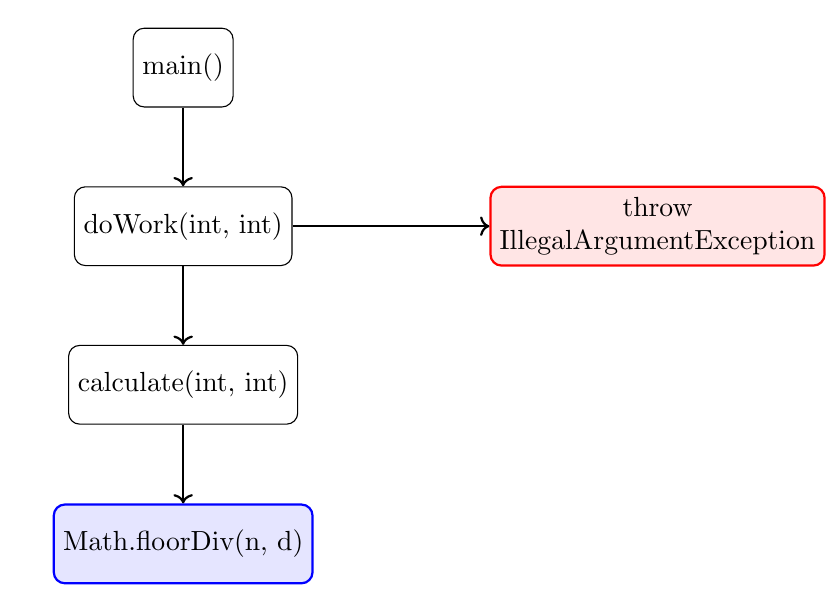
\begin{tikzpicture}[
    node distance=1cm and 2.5cm,
    every node/.style={draw, rounded corners, align=center, minimum height=1cm},
    exception/.style={draw=red, thick, rounded corners, align=center, minimum height=1cm, fill=red!10},
    libcall/.style={draw=blue, thick, rounded corners, align=center, minimum height=1cm, fill=blue!10},
    arrow/.style={->, thick}
]

% Nodes
\node (main) {main()};
\node (doWork) [below=of main] {doWork(int, int)};
\node (calculate) [below=of doWork] {calculate(int, int)};
\node[exception] (iae) [right=of doWork] {throw \\ IllegalArgumentException};
\node[libcall] (floorDiv) [below=of calculate] {Math.floorDiv(n, d)};

% Edges
\draw[arrow] (main) -- (doWork);
\draw[arrow] (doWork) -- (calculate);
\draw[arrow] (doWork) -- (iae);
\draw[arrow] (calculate) -- (floorDiv);

\end{tikzpicture}
\caption{Call graph for the \texttt{Example} program showing method calls and exception sources.}
\label{fig:callgraph-example}
\end{figure}

Figure~\ref{fig:callgraph-example} illustrates the call graph for the given Java program. The graph shows the sequence of method calls starting from the \texttt{main()} method, through \texttt{doWork()}, and into \texttt{calculate()}. Inside \texttt{doWork()}, a critical operations occur: a user-defined unchecked exception (\texttt{IllegalArgumentException}) is explicitly thrown when the denominator is zero.

This call graph is useful in tracing the flow of potential exceptions—both user-defined and library-sourced—through the client code. If a library version introduces a new unchecked exception at any point in this call chain (e.g., inside \texttt{Math.floorDiv()}), the static call graph can help identify all the client-side methods that may now be affected by that change. This is essential for detecting \glspl{bbc}.

\textbf{DUETS Dataset}. The DUETS dataset~\cite{durieux21:_duets} provides a list of real-world Java
client-library pairs. Each client in the DUETS dataset has over 5 stars on GitHub. For our evaluation,
we selected a convenience sample from the first few hundred clients in DUETS, rather than using the
entire dataset of 147,991 clients. The DUETS dataset provides a list of Java-based clients that are
more actively maintained and show better community engagement, as all the projects have over 5 stars.
It represents real-world library usage in Java-based projects.

\textbf{SootUp}. SootUp~\cite{Karakaya24:_SootUp} is a lightweight, modern Java framework built on top of Soot~\cite{vallee2010soot} that supports static analysis of Java bytecode.

SootUp transforms JVM bytecode into the intermediate representation Jimple~\cite{sootup}, which simplifies analysis by converting low-level bytecode instructions into a higher-level format that captures method bodies, variable assignments, exception handling blocks, and method invocations. SootUp also provides call graph generation with various algorithms and precision levels. We use the call graph to trace the propagation of exceptions from libraries to clients. When a library method throws a new unchecked exception, we use SootUp to determine whether client methods transitively call that library method by traversing the call graph. We also use the intermediate representation to inspect methods that may throw an exception by examining throw statements and method calls within their bodies.

%======================================================================
\chapter{Motivating Example}
%======================================================================

We present a motivating example to showcase how a newly added unchecked exception can cause a \gls{bbc} in the client code. We select the client/library pair from the DUETS dataset~\cite{durieux21:_duets}. We also demonstrate how we wrote a test case to verify the behavioural breaking change in the client caused by the updated library.

For this motivating example, we use \texttt{HttpAsyncClientUtils}\footnote{\url{https://github.com/iiweniiang/HttpAsyncClientUtils}} as our client. This client appears in the DUETS dataset. It declares version 4.4.6 of the \texttt{httpcore} library as one of its dependencies. Since the release of version 4.4.6, the developers of the \texttt{httpcore} library have released several newer versions. The latest available version is 4.4.16.\footnote{While \texttt{httpcore} 5.2.4 is in fact the latest version of this library, the library developers have released \texttt{httpcore5} as a distinct Maven component from \texttt{httpcore4}, and labelled \texttt{httpcore}(4) as end-of-life.}.

The update from version 4.4.6 to 4.4.16 of the \texttt{httpcore} library introduces a check for a new condition. In this update, the library checks the length of the argument provided by the client to the \gls{api}. Version 4.4.16 verifies whether the argument length is equal to "0", and if so, throws a new \texttt{IllegalArgumentException}. In the specific case of \texttt{HttpAsyncClientUtils} as the client and \texttt{httpcore} as the library, the client uses the \gls{api} method that includes this newly added check. We now demonstrate how UnCheckGuard identifies that the client is using a method from the library, detects the newly added exception, and verifies that the exception is actually triggerable by the client in order to avoid false positives.

\section{Detecting invocation of a library method in client}

A newly added unchecked exception in a library is only relevant to a client if the client actually uses the library method that introduces the exception. UnCheckGuard eliminates analysis of unused library methods by first analyzing the client for external method invocations. We perform this analysis by identifying all external method calls within the client code using Sootup~\cite{Karakaya24:_sootup}. In the case of \texttt{HttpAsyncClientUtils} as the client, it calls the \texttt{HttpCore} library from its public \texttt{createAsyncClient(boolean)}\footnote{Fully-qualified: method \texttt{createAsyncClient(boolean)} returning a \texttt{CloseableHttpAsyncClient} on class \texttt{Util.HttpClientUtil.HttpAsyncClient}.} method, which creates an \texttt{HttpHost} with an empty \texttt{host}. This method accepts a \texttt{proxy} parameter and includes the following code:

\begin{lstlisting}[language=Java]
 if (proxy) {
  return HttpAsyncClients.custom()
   .setConnectionManager(conMgr)
   .setDefaultCredentialsProvider(credentialsProvider)
   .setDefaultAuthSchemeRegistry(authSchemeRegistry)
   .setProxy(new HttpHost(host, port))
   .setDefaultCookieStore(new BasicCookieStore())
   .setDefaultRequestConfig(requestConfig).build();
 } else {
   // ...
\end{lstlisting}

The \texttt{HttpAsyncClientUtils} client declares the two variable (host and port) required for \texttt{HttpHost} (line 6 in the above code) in the following way:
\begin{lstlisting}[language=Java]
    private String host = "";
    private int port = 0;
   // ...
\end{lstlisting}

The client initializes \texttt{host}, a private field of type \texttt{String}, as an empty string and sets \texttt{port} to 0. As a result, the client calls \texttt{<init>(String, int)}\footnote{Specifically, constructor \texttt{<init>(String, int)} returning a \texttt{void} on class \texttt{org.apache.http.HttpHost}} with the host set to an empty string and the port set to 0.
% Thus, calling \texttt{createAsyncClient(true)} triggers an exception when executed with
% \texttt{httpcore} version 4.4.16 but not with 4.4.6.

After collecting all external method calls made by the client \texttt{HttpAsyncClientUtils}, UnCheckGuard begins comparing the version of the library currently used by the client with the latest available version. It stores all external method invocations made by the client—not just those to the \texttt{HttpHost} library in a \texttt{JSON} file. If UnCheckGuard detects a newly added exception in any of these external method calls, it then uses taint analysis to check whether the exception is actually reachable from the client. For this client, UnCheckGuard identifies a call to \texttt{HttpHost}. The next step for UnCheckGuard is to detect the newly added exception and verify its reachability.


% To detect that our \texttt{HttpAsyncClientUtils} client calls a method from \texttt{httpcore-4.4.6} which, upon upgrading to \texttt{httpcore-4.4.16}, may throw a new unchecked exception, UnCheckGuard begins by identifying all external library methods invoked anywhere in the client. It then analyzes both the current and the latest versions of the library to determine whether any newly introduced unchecked exceptions are reachable from the client's code. Here, reachability means that the client can trigger the exception in the library on some execution of the program, using values it passes to the library as parameters.

\section{Detecting newly added exception in Library} 

UnCheckGuard in the previous step found that the client \texttt{HttpAsyncClientUtils} makes a call to the constructors for the \texttt{org.apache.http.HttpHost} class. UnCheckGuard now analyzes the set of exceptions thrown by the constructor for both 4.4.6 and 4.4.16 version.

% To detect this change, UnCheckGuard processes JAR files for both \texttt{httpcore-4.4.6} and \texttt{httpcore-4.4.16}. It uses SootUp~\cite{Karakaya24:_sootup} to construct a call graph using Class Hierarchy Analysis (CHA) starting from the public \texttt{<init>(String, int)}\footnote{Specifically, constructor \texttt{<init>(String, int)} returning a \texttt{void} on class \texttt{org.apache.http.HttpHost}} constructor on \texttt{HttpHost} and identifies the set of all methods transitively reachable by the client (which we will discuss below). UnCheckGuard then collects all unchecked exceptions thrown within this set of reachable methods, for both library versions.
To determine whether the newer version of the library introduces a newly added exception, UnCheckGuard analyzes the JAR files for \texttt{httpcore-4.4.6} and \texttt{httpcore-4.4.16}. It performs this analysis using SootUp~\cite{Karakaya24:_sootup}. UnCheckGuard constructs a call graph using Class Hierarchy Analysis (CHA), starting from the public \texttt{<init>(String, int)} constructor in \texttt{HttpHost}. With the help of this call graph, UnCheckGuard identifies the set of all methods transitively reachable by the client (discussed below). It then collects the list of exceptions present within those methods. UnCheckGuard performs this process for both the currently used version of the library and the newer version. During this step, it stores the list of exceptions found in different methods of a particular \gls{api} in a \texttt{JSON} file, as this information is needed later for comparison.

Now, based on the call graph constructed for the public \texttt{<init>(String, int)} constructor on \texttt{HttpHost}, UnCheckGuard find that the constructor calls the static method \texttt{Args.containsNoBlanks()}\footnote{Fully-qualified name: method \texttt{containsNoBlanks(java.lang.CharSequence,java.lang.String)} returning a \texttt{java.lang.CharSequence} on class \texttt{org.apache.http.util.Args} } in the version 4.4.16.

% All constructors for the \texttt{org.apache.http.HttpHost} class transitively call
% the static method \texttt{Args.containsNoBlanks()}. Between version 4.4.6 and version 4.4.16, the \texttt{httpcore}
% developers added the following lines of code to \texttt{containsNoBlanks()}:

Upon a manual inspection of the static method \texttt{Args.containsNoBlanks()}, we find that the developers have added the following lines of code to the 4.4.16 version:

\begin{lstlisting}[language=Java]
  public static <T extends CharSequence> T containsNoBlanks(final T argument, final String name) {
        ...
        if (argument.length() == 0) {
            throw new IllegalArgumentException(name + " may not be empty");
        }
        ...
        return argument;
    }
\end{lstlisting}

Specifically, all \texttt{HttpHost} constructors take a \texttt{hostname} parameter and call \texttt{containsNoBlanks()}
with that parameter (to check that it contains no blanks). In the case when the length of the argument (\texttt{host}) is equal to zero it throws a unchecked exception \texttt{IllegalArgumentException}. A client can therefore trigger this newly added exception
in a client by attempting to instantiate a new \texttt{HttpHost} object and passing it an empty
\texttt{hostname}.

\begin{figure}[htbp]
    \centering
    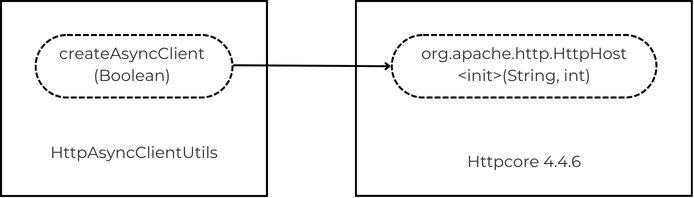
\includegraphics[width=0.6\textwidth]{diagram/httpcore6.png}
    \caption{External method call from \texttt{createAsyncClient(Boolean)} in \texttt{HttpAsyncClientUtils} to the \texttt{HttpHost} constructor \texttt{<init>(String, int)} in \texttt{Httpcore 4.4.6}.}
    \label{fig:httpcore6}
\end{figure}

\begin{figure}[htbp]
    \centering
    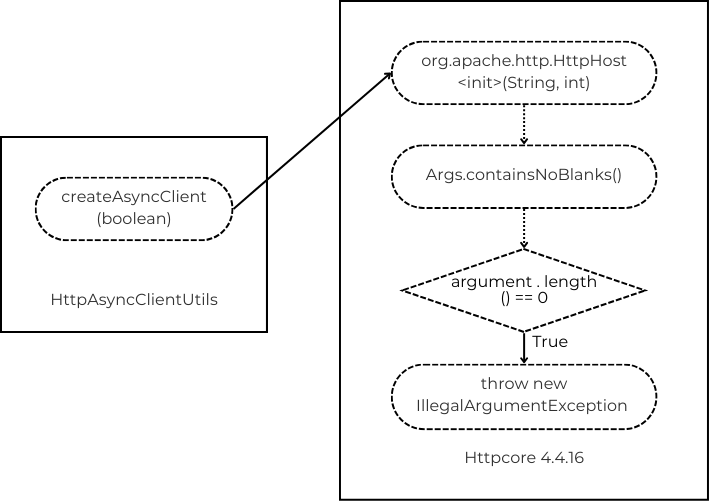
\includegraphics[width=0.75\textwidth]{diagram/httpcore16.png}
    \caption{External method call from \texttt{createAsyncClient(Boolean)} in \texttt{HttpAsyncClientUtils} to the \texttt{HttpHost} constructor \texttt{<init>(String, int)} in \texttt{Httpcore 4.4.16}, which internally validates arguments using \texttt{Args.containsNoBlanks()} and may throw an \texttt{IllegalArgumentException}.}
    \label{fig:httpcore16}
\end{figure}

Our UnCheckGuard tool analyzes the changes in \texttt{httpcore} and finds that, in version 4.4.16, all of the \texttt{HttpHost} constructors can now throw an \texttt{IllegalArgumentException} through the \texttt{containsNoBlanks()} method, as shown in Figure~\ref{fig:httpcore16}. Version 4.4.6 does not throw this exception, as shown in Figure~\ref{fig:httpcore6}. To further verify whether the client can actually trigger this exception, we apply taint analysis.

\section{Verifying if the client can trigger the exception}

% To verify if the client-supplied values can reach the exception-throwing site, we use taint analysis, as implemented using
% FlowDroid~\cite{Arzt14:_flowdroid}. Taint analysis is required in this scenario because the presence of a control-flow
% path from the client callsite to an exception-throwing statement is not sufficient to conclude that the exception is actually
% triggerable by the client. We found that many such paths may exist in a library, but the path conditions leading to the
% exception might depend entirely on internal library values, rather than on client-supplied inputs; it is impossible for our
% client to cause the execution of any path that triggers the exception. In our experience, taint analysis can help distinguish
% actual behavioural breaking changes from false positives.

After UnCheckGuard collects the methods that introduce newly added exceptions in the latest version of the library, it verifies whether the client-supplied values can actually trigger those exceptions. UnCheckGuard checks whether the client-supplied values can reach the exception-throwing site. To perform this verification, UnCheckGuard applies taint analysis using FlowDroid~\cite{Arzt14:_flowdroid}. Taint analysis is necessary in this situation because the presence of a control-flow path between the client callsite and the exception-throwing statement is not sufficient to conclude that the exception is actually triggered by the client. In many scenarios, such a path may exist in the library, but the path condition leading to the exception may depend entirely on internal library values rather than on client-supplied input; in these cases, the client cannot cause the execution of any path that throws the exception. In our experience, taint analysis proves beneficial in distinguishing actual behavioural breaking changes from false positives. In the methodology section, we provide an example of a library that introduces a newly added exception, but the exception is not triggerable with the client-supplied values.


% Specifically, we use taint analysis to track whether any client-supplied method parameters to library calls (source) can propagate to the exception object's constructor (sink). If taint analysis determines that no client-supplied input flows into the exception-triggering logic, then we can conclude that the newly added exception will not cause a behavioural breaking change, and we do not report that exception.
%For exceptions that we report, we know that a path exists in the interprocedural control-flow graph (which one can compute with CHA) from the client method to the statement throwing the exception in the library.

Taint analysis tracks whether any client-supplied values to the external method used by the client can reach the exception object's constructor. UnCheckGuard marks the client-supplied values as \texttt{SOURCE} and the exception object's constructor as \texttt{SINK}. If taint analysis determines that the \texttt{SOURCE} cannot reach the \texttt{SINK}, or that the \texttt{SOURCE} cannot flow into the exception-triggering logic, then UnCheckGuard does not report the case to the client, as the newly added exception will not result in a behavioural breaking change.

UnCheckGuard marks the following as \texttt{SOURCE}:
\begin{itemize}
  \item \texttt{hostname}
  \item \texttt{port}
\end{itemize}

UnCheckGuard marks the following as the \texttt{SINK}:
\begin{itemize}
  \item \texttt{IllegalArgumentException} found in \texttt{Args.containsNoBlanks()}
\end{itemize}

In version 4.4.6, UnCheckGuard finds two sites throwing \texttt{IllegalArgumentException}, while in 4.4.16, it detects three—each of which the client can potentially trigger using the values it chooses to pass to the library as parameters.

Based on FlowDroid's confirmation of the reachability of the new exception's constructor, we report that the library-client pair \texttt{HttpAsyncClientUtils} and \texttt{httpcore} exhibits a behavioural breaking change.

Given this report from UnCheckGuard, it is straightforward to write a test case that calls the client's \texttt{createAsyncClient()} method
and triggers the exception after an upgrade:
\begin{lstlisting}[language=Java]
@Test
void testCreateAsyncClientThrowsExceptionForEmptyProxyHost() {
  HttpAsyncClient client = new HttpAsyncClient();

  IllegalArgumentException exception =
    assertThrows(IllegalArgumentException.class, () -> {
        client.createAsyncClient(true);
    });

    assertTrue(exception.getMessage()
    .contains("may not be empty"),
      "Expected exception due to empty hostname "+
      "after upgrading to httpcore-4.4.16");
}
\end{lstlisting}

The above test case passes for version 4.4.16 of \texttt{Httpcore}, as the constructor method of \texttt{org.apache.http.HttpHost} throws an \texttt{IllegalArgumentException} when called with an empty \texttt{hostname}. The same test case fails for version 4.4.6 of \texttt{Httpcore}, as this version does not contain the exception.

This test case\footnote{Link for the test case: \url{https://github.com/vinayaksh42/HttpAsyncClientUtils/blob/new/src/test/java/Util/HttpClientUtil/HttpAsyncClientTest.java}} demonstrates how a \texttt{PATCH} version upgrade (from 4.4.6 to 4.4.16) can introduce a behavioural breaking change due to a newly added exception. Further, it also demonstrates how UnCheckGuard operates.

%======================================================================
\chapter{Data Collection}\label{data}
%======================================================================
% This section describes the systematic approach we used to construct the dataset for our study on behavioural incompatibilities caused by newly added unchecked exceptions in upgraded Java libraries. 

This chapter describes the approach we use to construct the dataset for our study on behavioural incompatibilities caused by newly added unchecked exceptions in upgraded Java libraries. The data we collect creates the foundation for our analysis in subsequent chapters. Specifically, it enables UnCheckGuard to detect methods that introduce newly added unchecked exceptions, identify affected client call sites (Chapter~\ref{methodology}).

% Broadly, we require three sets of components: Java-based clients that depend on third-party libraries; the versions of the libraries declared as dependencies by these clients (``current'' versions); and the latest available versions of those same libraries (``latest'' versions). For each client-library pair, we also need to extract the set of unchecked exceptions thrown by the library methods actually used by the client.

The tool UnCheckGuard requires three components to perform its analysis: Java-based clients that depend on third-party libraries; the versions of the libraries these clients currently declare as dependencies (“current” versions); and the latest available versions of those same libraries (“latest” versions). For each client, the tool extracts the unchecked exceptions thrown by both the current and the latest versions of the library. It then formulates a list of methods that, when upgraded to the newer version, introduce a newly added unchecked exception. The tool focuses on extracting and storing this information only for the methods that the client application actually uses.

% To collect data that our UnCheckGuard tool will use, we carry out the following steps: identifying suitable Java clients; extracting their library dependencies; resolving both the current and latest versions of the libraries; analyzing exception behaviour in both versions; and recording all methods that introduce newly added unchecked exceptions. Using this data, UnCheckGuard can report client call sites that may be affected by behavioural breaking changes in a library upgrade.

To collect the data mentioned above, our tool UnCheckGuard follows these steps:
\begin{itemize}
    \item Identify suitable Java clients.
    \item Extract their library dependencies and resolve both the current and latest versions of the libraries.
    \item Extract methods for analysis.
    \item Record all methods that introduce newly added unchecked exceptions.
\end{itemize}
With this data, UnCheckGuard reports the call sites present in the client application that may be affected by behavioural breaking changes during a library upgrade.

\section{Collecting Clients}

% To begin our analysis, we first collected suitable client projects. We used the DUETS dataset~\cite{durieux21:_duets}, which provides a curated list of Java-based clients hosted on GitHub, each with at least five stars. DUETS also pairs libraries with the clients, but we ignore the DUETS library declarations and instead consider all of the libraries declared as dependencies by each client.

To start our analysis, we created a \texttt{Python} script to collect suitable client projects. For this process, we used the DUETS dataset~\cite{durieux21:_duets}, which provides a curated list of Java-based clients hosted on GitHub. We selected this list because all Java projects in it have at least 5 stars on GitHub. The DUETS dataset includes projects with a minimum of 5 stars, as this indicates a baseline level of community engagement; stronger engagement generally reflects a more actively maintained project. This helps us collect clients that represent real-world library usage in Java-based projects.

% We took a convenience sample of the first few hundred clients from DUETS rather than the entire DUETS dataset of 147,991 clients. We attempted to download each client repository and discarded any client that failed to download.

% Next, we checked whether the project included a \texttt{pom.xml} file, which indicates that it is a Maven-based project. This step was essential, as our analysis depends on running Maven commands. We compiled each client to produce a JAR file and kept only those clients that compiled successfully for further analysis. After this process, we were left with 36 Maven-based clients that we had successfully compiled.

We ran our \texttt{Python} script on the first few hundred clients from the DUETS dataset, rather than on the entire dataset of 147,991 clients. We attempted to download each client repository and discarded any client that failed to download. 

Next, we checked whether the project included a \texttt{pom.xml} file; the presence of this file indicates that the project is Maven-based. We discarded any project that was not Maven-based, as our analysis depends on running Maven commands. The \texttt{Python} script then checked the Java version specified in the \texttt{pom.xml} file, and based on that version, we ran the Maven commands using the corresponding Java environment. We compiled each client to produce a JAR file and retained only those clients that compiled successfully for further analysis. After completing this filtering process, we were left with 36 Maven-based clients that we had successfully compiled.


\section{Library Version Resolution}

% Our tool relies on analyzing both the version of the library currently used by the client and the latest available version (as stored in the Maven Central Repository). To collect the current version, we run the Maven command \texttt{mvn dependency:copy-dependencies}, which downloads all the dependencies declared in the client's build configuration.

UnCheckGuard depends on analyzing both the current version of the library used by the client and the latest available version of the library, as stored in the Maven Central Repository. To collect both versions, we run a set of Maven commands. To retrieve the current version of the library, we run the following set of Maven commands:

\begin{lstlisting}[language=bash]
mvn clean package -DskipTests -fn
mvn dependency:copy-dependencies
\end{lstlisting}

This command allows us to store all the dependencies currently used by the client.

To obtain the latest version of the libraries, we run the following Maven command:
\begin{lstlisting}[language=bash]
mvn org.codehaus.mojo:versions-maven-plugin:2.18.0:use-latest-versions
mvn clean package -DskipTests -fn
mvn dependency:copy-dependencies
\end{lstlisting}
This command updates the \texttt{pom.xml} file with the most recent versions of all declared dependencies. We then re-run \texttt{mvn dependency:copy-dependencies} to download the updated set of libraries.

This process fetches both the current and the latest versions of each library used by the client, enabling us to perform a comparative analysis of behavioural changes across library versions. Out of the 36 clients that we collected, we found 26 clients with different current and latest versions for some library. These clients collectively used 17 libraries with different versions, with 22 current versions used by some client, updated to 17 latest versions.

\section{Method Extraction}

% We analyze the JAR file of the client application using SootUp~\cite{Karakaya24:_SootUp} to extract all external method invocations performed by the client (by external, we mean to methods outside the client). Based on this set of method calls, we analyze both the version of the library that the client currently uses as well as its latest available version.

UnCheckGuard then begins analyzing the clients we collected in the first step. It uses SootUp~\cite{Karakaya24:_SootUp} to extract all external method invocations. By external methods, we mean methods that are not defined within the client's own codebase—methods whose definitions reside in third-party libraries. We store a list of all external method invocations made by the client in a \texttt{JSON} file. This file is later used to compare against the different methods within the libraries that the client uses.

To support this comparison, we extract the list of methods present in the current version of the library. This allows us to match each external method call made by the client to its corresponding definition in the library. Using this information, we generate a JSON file that contains only the subset of library methods actually used by the client. This filtered list reduces the work necessary in subsequent steps.


\section{Comparing Library Versions}

UnCheckGuard then analyzes the methods used by the client in both the current and the latest available versions of the library. The tool scans for exceptions and performs taint analysis to verify the reachability from the client to the exceptions present in the method. After collecting the unchecked exceptions from both versions of the library, we store the list of exceptions present in each method in a \texttt{JSON} file. We use the following format to store this information:
\begin{lstlisting}[language=python]
[
    ...
    {"org.apache.http.HttpHost": [{
        "methodSignature": "<org.apache.http.HttpHost: void <init>(java.lang.String,int)>",
        "unchecked_exceptions": [
            "java.lang.IllegalArgumentException <org.apache.http.util.Args: java.lang.CharSequence containsNoBlanks(java.lang.CharSequence,java.lang.String)>",
            "java.lang.IllegalArgumentException <org.apache.http.util.Args: java.lang.CharSequence containsNoBlanks(java.lang.CharSequence,java.lang.String)>"
        ]
    }]},
    ...
]
\end{lstlisting}

This \texttt{JSON} file contains a list of classes in the library. For each class, it includes a list of methods, and for each method, it stores two fields: \texttt{methodSignature}, which holds the method’s signature, and \texttt{unchecked\_exceptions}, which lists all unchecked exceptions associated with the method. The tool uses this \texttt{JSON} file to compare the current and latest versions of the library. We remove any duplicate exceptions that appear in both versions. If a method in the latest version throws an exception not present in the older version, we tag that method as having a newly added unchecked exception. Note that our methodology does not detect cases where a method throws the same exception but under new conditions.

% Our tool detects newly added unchecked exceptions by scanning method implementations, and approximates their reachability from the client using taint analysis. After collecting the unchecked exceptions from both the current and the latest versions of the library, we compare the sets of exceptions associated with each method in the library. We remove any duplicate exceptions that appear in both versions. If a method in the latest version throws an exception that was not present in the older version, we tag that method as having a newly added unchecked exception. Note that our methodology does not detect instances where the same exception is thrown by a method, but under new circumstances.

This output enables our tool to highlight call sites in the client application that may exhibit behavioural breaking changes, helping developers assess the impact of upgrading their dependencies.


%======================================================================
\chapter{Methodology}\label{methodology}
%======================================================================
The last chapter, Chapter~\ref{data}, described how we collected the clients and libraries, as well as the necessary information to perform our analysis. In this section, we describe our methodology for detecting and verifying newly added unchecked exceptions in a library when it is updated from an older version to a newer one. Our focus is on identifying the impact of such changes on client code. Specifically, we analyze client programs to detect usage of library methods that were updated to throw previously non-existent unchecked exceptions. Java distinguishes between checked exceptions, which appear as part of method signatures, and unchecked exceptions, which do not. Unchecked exceptions may therefore introduce a class of breaking changes that method signature-based syntactic approaches for Java cannot detect.

After carrying out the data collection steps in Chapter~\ref{data} and extracting all external library methods invoked by the client, we next analyze their implementations, in both the current version and the latest version. This allows us to compare their behaviour across versions. Our analysis is specifically targeted at detecting one particular class of behavioral breaking changes: the introduction of new unchecked exceptions in updated library methods that the client can trigger with the client-supplied values. If we find, through our analysis, that a method now throws a newly added unchecked exception in the latest version, and that the exception can be triggered from the client code, we flag a potential behavioural breaking change. To verify whether this change is in fact breaking, we currently manually write test cases to verify that the client may be affected by the newly introduced exception. We found that this was easy to do given the information that UnCheckGuard reports. 

\section{Problem Definition}

Let $P$ be a Java client program that depends on a library $L$ at version $v_{old}$, and suppose that $L$ is later updated to version $v_{new}$. We wish to determine whether any methods in $L$ now throw \textit{new unchecked exceptions} in $v_{new}$ that did not occur in $v_{old}$, and whether such exceptions can be triggered by valid usage patterns in $P$.

Formally, given:
\begin{itemize}
  \item A client program $P$, compiled as a JAR file;
  \item A library $L$ in two versions: $L_{old}$ and $L_{new}$;
  \item A set of method invocations from $P$ to $L$, denoted $\texttt{Calls}(P \rightarrow L)$;
\end{itemize}

Our task is to identify a set of pairs $(m, e)$ where:
\begin{itemize}
  \item $m$ is a method in $L$ that is invoked by $P$;
  \item $e$ is a subclass of \texttt{java.lang.RuntimeException} or \texttt{java.lang.Error};
  \item $e$ is not thrown (transitively) by $m$ in $L_{old}$, but is thrown in $L_{new}$;
  \item There exists a path from a client-controlled input in $P$ to the exception site where $e$ is instantiated.
\end{itemize}

We refer to such pairs as \textit{client-reachable newly added unchecked exceptions}, and consider them potential behavioural breaking changes.

Note that we focus exclusively on \textbf{unchecked} exceptions, which do not appear in Java method signatures. Checked exceptions are excluded from this study as they are already caught by signature-diffing tools such as japicmp.

\section{Analysis Setup}

\begin{figure*}[hbt!]
    \centering
    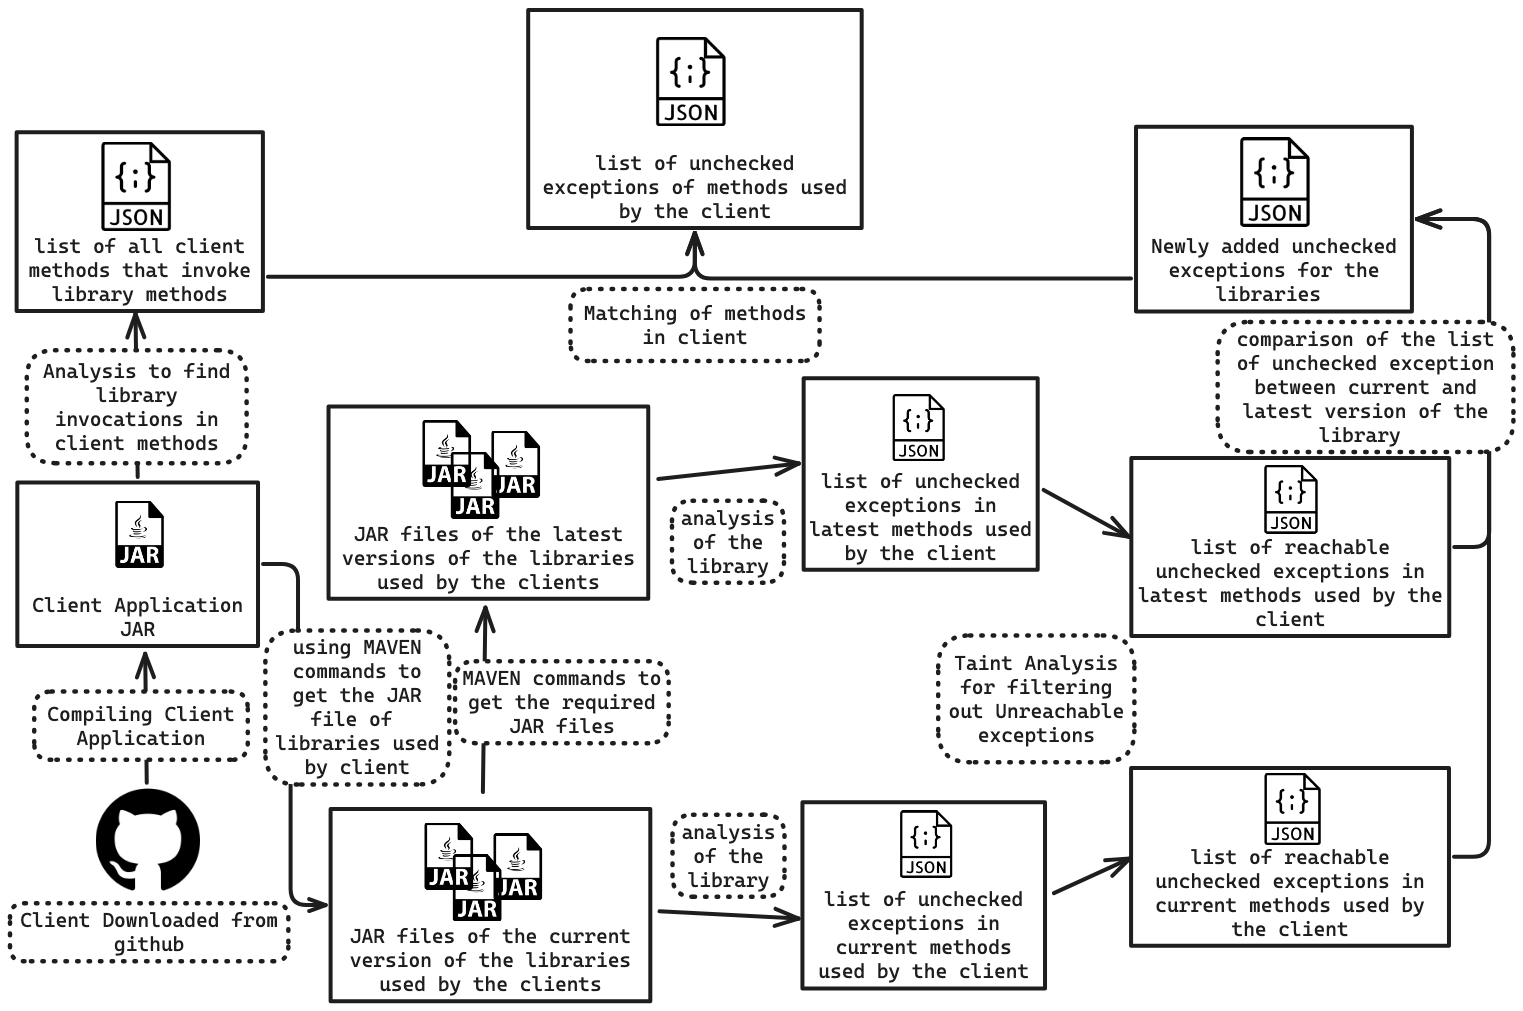
\includegraphics[height=260pt]{diagram/finalfpioeline.png}
    \caption{Pipeline of UnCheckGuard for detecting behavioural breaking changes due to newly added unchecked exceptions.}
    \label{fig:jsonjava}
\end{figure*}

We divide analysis setup into two steps: 1) library version resolution; and 2) mapping external method invocations to library methods. Figure~\ref{fig:jsonjava} shows the full pipeline.

As described in Chapter~\ref{data}, we begin by selecting Java-based clients from the DUETS dataset~\cite{durieux21:_duets}. We retain only those clients that are Maven-compatible and successfully compile to a JAR file, ensuring compatibility with our analysis tooling.

After selecting the valid clients and compiling them into JAR files, we proceed to extract relevant method-level knowledge from both the client and the current version of the libraries it depends on.

\subsection{Library Version Resolution}

% Our tool relies on analyzing both the version of the library currently used by the client and the latest available version (as stored in the Maven Central Repository). To collect the current version, we run the Maven command \texttt{mvn dependency:copy-dependencies}, which downloads all the dependencies declared in the client's build configuration.

UnCheckGuard depends on analyzing both the current version of the library used by the client and the latest available version of the library, as stored in the Maven Central Repository. To collect both versions, we run a set of Maven commands. To retrieve the current version of the library, we run the following set of Maven commands:

\begin{lstlisting}[language=bash]
mvn clean package -DskipTests -fn
mvn dependency:copy-dependencies
\end{lstlisting}

This command allows us to store all the dependencies currently used by the client.

To obtain the latest version of the libraries, we run the following Maven command:
\begin{lstlisting}[language=bash]
mvn org.codehaus.mojo:versions-maven-plugin:2.18.0:use-latest-versions
mvn clean package -DskipTests -fn
mvn dependency:copy-dependencies
\end{lstlisting}
This command updates the \texttt{pom.xml} file with the most recent versions of all declared dependencies. We then re-run \texttt{mvn dependency:copy-dependencies} to download the updated set of libraries.

This process fetches both the current and the latest versions of each library used by the client, enabling us to perform a comparative analysis of behavioural changes across library versions. Out of the 1011 clients that we collected, we found that these clients collectively used 302 libraries.

\subsection{Mapping External Method Invocations to Library Methods}

We use SootUp~\cite{Karakaya24:_SootUp} to analyze the client JAR and identify all external method invocations. By external methods, we mean methods that are not defined within the client’s own codebase—methods whose definitions reside in third-party libraries. UnCheckGuard performs this analysis by traversing the Jimple intermediate representation of each client method and checking whether any statement contains an \texttt{InvokeExpr}, which represents a method invocation. For each invocation, we retrieve the declaring class type of the target method. We then check whether this class type is part of the client’s SootUp view---essentially, whether it was declared in the client JAR file or the Java standard library. If the class type is not found in the view, we mark the method as external. This process allows us to filter out internal method calls and consider only invocations to external library methods.

In parallel, we analyze the current version of each library used by the client. We extract all method signatures defined in the library JAR. We then match each external method call made by the client to the corresponding method in the library, by comparing their fully qualified method signatures. For the matching process, for simplicity, we perform an exact match between the declaring type of the method invoked by the client and that in the library to create a client/library mapping. This approach may miss some valid matches in the presence of dynamic dispatch---the declared receiver object type may differ from the actual receiver object type that the client uses at the call site---so the current version of UnCheckGuard may underreport some breaking changes.

Our client/library mapping identifies library methods and links them to where they can be invoked by the client. This mapping serves as a foundation for later stages in our analysis, where we detect behavioural changes in the latest versions of libraries and traces their potential impact on client call sites.


\section{Finding Newly Added Unchecked Exceptions}

Our primary goal is to detect whether upgrading a library introduces new unchecked exceptions that could affect client behaviour. To achieve this, we divide the process into two stages: first, identifying newly added unchecked exceptions using a call graph; and second, verifying their reachability from client input using a taint analysis. We then compute differences between versions in the sets of reachable exceptions.

\subsection{Exception Discovery}

To detect newly added unchecked exceptions in the latest library versions, we first construct a call graph using SootUp's Class Hierarchy Analysis implementation. CHA includes all methods with the correct signature defined in subclasses and interface implementations.

%We use RTA instead of Class Hierarchy Analysis (CHA) because RTA provides a more precise approximation of runtime behaviour in the context of a particular client/library pair. RTA instead considers only those types that are instantiated in the program (client plus libraries), resulting in a more accurate call graph.

By definition, CHA reports the most conservative soundy~\cite{livshits15:_in} answer possible, absent reflection and other dynamic features. Thus, it tends to over-approximate, reporting method calls that are unreachable in practice. For example, in one case, CHA identified a path from the public \texttt{getString(String)}\footnote{Fully-qualified name: method \texttt{getString(String)} returning a \texttt{String} on class \texttt{com.alibaba.fastjson.JSONObject}} method, reporting an exception thrown in the \texttt{JSONObject} constructor as reachable. However, manual inspection revealed that this path was spurious—the method \texttt{getString} never reaches the constructor in question because, in the specific program under analysis, no code instantiates a \texttt{JSONObject}. Our next step, taint analysis, filters out some such unreachable methods.

%RTA excludes such paths because it considers only types that are actually instantiated, whereas CHA includes all potential subtype relationships, regardless of runtime feasibility.
% we should probably make this whole discussion more concise when we have space limitations

We traverse our callgraph and collect all instantiated exceptions that are subclasses of either \texttt{java.lang.RuntimeException} or \texttt{java.lang.Error}. Per the definition of the Java programming language, such exceptions represent the complete set of unchecked exceptions that the client might be newly exposed to due to the library upgrade.

\subsection{Exception Filtering with Taint Analysis}

Once we collect the list of unchecked exceptions, we need to determine which of them can actually be triggered by client inputs. This is necessary because many exceptions that show up during call graph analysis are not reachable in practice—they rely on internal values rather than any parameters the client supplies (see below for an example). To filter out such cases, we use FlowDroid~\cite{Arzt14:_flowdroid}, a static taint analysis framework.

Consider the following case from our corpus. The client \texttt{4ntoine/ServiceDiscovery-java}\footnote{\url{https://github.com/4ntoine/ServiceDiscovery-java}} uses the method \texttt{copyFromUtf8(String)} from the library \texttt{protobuf-java-2.6.1}. This method, in turn, reaches the internal method \texttt{newInstance} in its call graph. When the library is upgraded to \texttt{protobuf-java-4.30.1}, the implementation of \texttt{newInstance} introduces a new unchecked exception—an \texttt{IllegalArgumentException}. Our tool initially flags this as a behavioural breaking change because the exception is newly introduced, and an interprocedural control-flow path exists from the client code to the exception site.

However, a closer inspection shows that this exception cannot be triggered by any value passed from the client. The internal method that throws the exception looks like this:

\begin{lstlisting}[language=Java,breaklines=true,basicstyle=\scriptsize\ttfamily]
static CodedInputStream newInstance(
    final byte[] buf, final int off, final int len, final boolean bufferIsImmutable) {
  ArrayDecoder result = new ArrayDecoder(buf, off, len, bufferIsImmutable);
  try {
    result.pushLimit(len);
  } catch (InvalidProtocolBufferException ex) {
    // The only reason pushLimit() might throw an exception
    // here is if len is negative. Normally pushLimit()'s
    // parameter comes directly off the wire, so it's 
    // important to catch exceptions in case of corrupt or
    // malicious data. However, in this case, we expect 
    // that len is not a user-supplied value, so we can 
    // assume that it being negative indicates a 
    // programming error. Therefore, throwing an unchecked 
    // exception is appropriate.
    throw new IllegalArgumentException(ex);
  }
  return result;
}
\end{lstlisting}

The library developer's comment states that this exception will never be thrown by this non-public method, essentially because \texttt{len} cannot be directly supplied by a client. Clients can only reach this \texttt{newInstance} method through methods that are part of \texttt{protobuf}'s public API. Our taint analysis confirms that no client-supplied value (source) flows into the \texttt{IllegalArgumentException} constructor (sink). We choose exception constructors as sinks because taintedness of the exception constructor means that the client-controlled value can affect the reachability of the exception, i.e. whether the exception might be thrown or not. Hence, taint analysis helps reason about whether the newly-added exception can actually cause a behavioural breaking change in the client.

We mark an exception site as \emph{reachable} if either the client-supplied value is used as an argument for the exception constructor (explicit) or the client-supplied value influences the control flow reaching the \texttt{throw} statement (implicit). This approach ensures that we correctly identify both explicit data dependence and implicit control-flow dependence on the client-supplied value.
Figure~\ref{fig:taint-flow} illustrates these two ways that client-supplied values can reach an exception site.

\begin{figure*}[t]
\centering
\resizebox{\textwidth}{!}{%
\begin{tikzpicture}[
  node distance=1.0cm and 1.2cm,
  >=Latex,
  box/.style={draw, rounded corners, align=center, minimum width=2.4cm, minimum height=0.9cm, inner sep=4pt},
  legend/.style={draw, rounded corners, align=left, inner sep=3pt},
  dataedge/.style={->, thick, shorten >=2pt, shorten <=2pt},
  ctrledge/.style={->, dashed, thick, shorten >=2pt, shorten <=2pt}
]
\node[box] (client) {Client\\ \texttt{caller(a)}\\ \textbf{Source}};
\node[box, right=of client] (call) {Call site\\ \texttt{lib.m(a)}};
\node[box, right=of call] (lib) {Library\\ \texttt{m(x)\{...\}}};
\node[box, below=1.0cm of lib, minimum width=3.2cm] (cond) {Branch\\ \texttt{if (g(x)) throw E(...)}};
\node[box, right=1.1cm of lib, minimum width=3.3cm] (ctor) {Exception constructor\\ \texttt{new E(...)}\\ \textbf{Sink}};
\node[box, right=of ctor, minimum width=2.0cm] (throw) {\texttt{throw e;}};

\draw[dataedge] (client) -- node[above]{taint} (call);
\draw[dataedge] (call) -- node[above]{\texttt{x:=a}} (lib);
\draw[dataedge] (lib)
  to[out=12,in=168]
  node[pos=0.55, above=4pt, sloped, fill=white, inner sep=1pt] {\texttt{msg := f(x)}}
  (ctor);

\draw[ctrledge] (lib) -- (cond);
\draw[ctrledge] (cond) to[out=25,in=-155] (ctor);
\draw[dataedge] (ctor) -- (throw);

\node[legend, anchor=south east] (leg) at (current bounding box.south east) {\textbf{Legend:}\\[-2pt]
\begin{tikzpicture}[baseline={(0,0)}]
  \draw[->, thick] (0,0) -- (1.0,0) node[right, xshift=6] {data dep.};
  \draw[->, dashed, thick] (0,-0.45) -- (1.0,-0.45) node[right, xshift=6] {control dep.};
\end{tikzpicture}
};
\end{tikzpicture}%
}
\caption{Taint propagation from a client parameter (source) to an exception site (sink) occurs via either \emph{data dependence} (solid lines, e.g., a value passed into the exception constructor arguments) or \emph{control-flow dependence} (dashed lines, e.g., a value influencing a branch that leads to the \texttt{throw} statement).}
\label{fig:taint-flow}
\end{figure*}


For technical reasons related to FlowDroid, we automatically generate a \textit{driver stub} for each value that the client supplies to the library. FlowDroid does not allow method parameters to be marked directly as taint sources. To work around this, we wrap each parameter in a synthetic method and mark its return value as a source.

This approach allows us to simulate tainted inputs and track their flow through the library method. Stub generation, implemented using SootUp, handles a variety of cases, including:
\begin{itemize}
  \item Constructor methods (\texttt{<init>} using \texttt{new ClassName(...)})
  \item Static and instance methods
  \item Void and non-void return types
  \item Primitive parameters (e.g., \texttt{int} $\rightarrow$ \texttt{0})
  \item Object parameters (defaulted to \texttt{null})
  \item Nested classes (converting \texttt{\$} to \texttt{.})
  \item Multiple parameters (sources named \texttt{SourceN()}, where $N$ is the parameter index)
  \item Overloaded methods (only one version retained)
\end{itemize}

An example of a driver stub follows.
\begin{lstlisting}[language=Java]
public class DriverStub {
    public static java.lang.String source0() {
        return null;
    }

    public static void run() {
        int result = new com.alibaba.fastjson.JSONObject().getIntValue(source0());
    }
}
\end{lstlisting}

In the above example of the driver stub, we generate a stub for library \texttt{fastjson-} \texttt{1.2.58}'s public \texttt{getIntValue(String)} method\footnote{Fully-qualified name: method \texttt{getIntValue(String)}, returning a \texttt{int} on class \texttt{com.alibaba.fastjson.JSONObject}}. This method has a \texttt{java.lang.String} parameter. We therefore declare a method named \texttt{source0} in the driver stub, and declare that method to be a source; FlowDroid then marks its return value as a source. We generate the way \texttt{getIntValue} is called based on the type of method it is, and obtain the properties of the method using SootUp.


In our analysis, we mark the parameters of library methods that are invoked by the client as taint sources (in the example in Chapter~\ref{example}, the \texttt{HttpHost} constructor parameters), since these are the only values under the client’s control. We also mark each exception identified in the Analysis Setup step as a potential taint sink. We use the taint analysis to estimate whether the client-supplied parameter values can trigger newly introduced exceptions. If they cannot, then the exception is effectively unreachable from the client, and thus does not constitute a behavioural breaking change. 


% I think we don't need to talk about this anymore
%% We treat each exception discovered in the RTA phase as a \textit{taint sink}. For this analysis, we intentionally construct the call graph using Class Hierarchy Analysis (CHA). Although CHA is less precise than RTA, it offers conservative coverage, reducing the risk of missing true positive flows due to aggressive pruning.

Consider the following method from the \texttt{beam-sdks-java-core} library:

\begin{lstlisting}[language=Java]
public static void applicableTo(PCollection<?> input) {
 WindowingStrategy<?, ?> ws = input.getWindowingStrategy();
 if (ws.getWindowFn() instanceof GlobalWindows
     && ws.getTrigger() instanceof DefaultTrigger
     && input.isBounded() != IsBounded.BOUNDED) {
  throw new IllegalStateException("...");
 }
}
\end{lstlisting}
%% \begin{figure}[t]
%% \centering
%% \scalebox{0.75}{
%% \begin{tikzpicture}[
%%   node distance=1.4cm and 1.5cm,
%%   box/.style={rectangle, draw, rounded corners, minimum height=1.2em, text width=2.8cm, align=center, font=\scriptsize},
%%   every edge/.style={draw, -{Latex[width=2mm]}},
%%   rededge/.style={draw=red, thick, dashed, -{Latex[width=2mm]}}
%%   ]

%% % Nodes
%% \node[box] (start) {\textbf{Method Entry}\\ \texttt{applicableTo(...)}};
%% \node[box, below=of start] (cond) {\textbf{Condition}\\ \texttt{input.isBounded() != BOUNDED}};
%% \node[box, below left=of cond] (exc) {Throws \\ \texttt{IllegalStateExcep...}};
%% \node[box, below right=of cond] (noexc) {Execution continues};

%% % Edges
%% \path (start) edge (cond);
%% \path (cond) edge (exc);
%% \path (cond) edge (noexc);

%% % Labels
%% \node[align=left, font=\scriptsize] at ([xshift=1.9cm,yshift=0.1cm]cond.east) {\textbf{CHA:} includes both branches};
%% \draw[rededge] (start.east) to[out=10,in=90] node[right, align=center, font=\scriptsize] {\textbf{RTA:} skips method due to\\ uninstantiated classes} (noexc.west);

%% \end{tikzpicture}
%% }
%% \vspace{-1ex}
%% \caption{CHA vs. RTA: RTA only reaches the \texttt{IllegalStateException} if types like \texttt{GlobalWindows} or \texttt{DefaultTrigger} are instantiated in the analyzed code.}
%% \label{fig:rta-vs-cha}
%% \vspace{-2ex}
%% \end{figure}


In this example, the parameter \texttt{input} is the taint source, and the \texttt{new IllegalState\\Exception()} is the sink (to be precise, the exception's constructor). The public \texttt{applicab\\leTo(PCollection)}\footnote{Fully-qualified name: method \texttt{applicableTo(PCollection)} returning a \texttt{void} on class \texttt{org.apache.beam.sdk.transforms.GroupByKe}} method is used by the \texttt{0xdecaf/beam-enrichment-patterns}\footnote{\url{github.com/0xdecaf/beam-enrichment-patterns}} client.

%% RTA excludes types that are never instantiated in the analyzed program. It is more precise and reaches the exception only if actual runtime types lead to the throw statement. In contrast, CHA is more conservative. In this case, RTA reaches the \texttt{IllegalStateException} only if classes such as \texttt{GlobalWindows} or \texttt{DefaultTrigger} are instantiated in the analyzed codebase. CHA, on the other hand, includes all possible overrides regardless of whether those types are instantiated. As a result, even if the actual runtime types are unused, CHA still explores all feasible paths and reaches the IllegalStateException. As shown in Figure~\ref{fig:rta-vs-cha}, this broader approximation allows taint analysis to identify exception flows that RTA would miss due to its stricter instantiation-based filtering.\todo{I still don't believe this: if GlobalWindows or DefaultTrigger are never invoked, why does it matter?}

% RTA excludes types that are never instantiated in the analyzed program. As a result, if no code in the client or the library instantiates a \texttt{PCollection}, the method \texttt{applicableTo(PCollection)} may not appear in the RTA-generated call graph at all. This exclusion causes the exception thrown in that method to be missed. In contrast, CHA includes all types from the class hierarchy regardless of instantiation, so the method is included in the call graph along with the conditional path to the exception. As shown in Figure~\ref{fig:rta-vs-cha}, this broader approximation allows the taint analysis to identify exception flows that RTA would miss due to its stricter instantiation-based filtering.

%% This trade-off justifies the use of CHA in the filtering phase: although it may over-approximate in some cases, it ensures that no critical exception flows are missed.

In terms of our methodology, for methods that appear in both the current and latest versions of the library, we compare the sets of unchecked exceptions that they throw, filter using taint analysis, and then diff to identify new exceptions (in the next stage). So, if the current version has unreachable exception E which becomes reachable in the latest version, but E was present in both versions, then we report E. (If a \emph{method} exists in the current library version but is missing from the latest version, we exclude it from our analysis. Its removal may indicate a method signature-based breaking change, but those are handled by existing tools and lie outside the scope of our detection. Our work only detects changes to the set of exceptions that are thrown.)

We compare exceptions using both the exception type (e.g., \texttt{java.lang.Illegal\\ArgumentException}) and the fully-qualified signature of the method in which the exception occurs. If, after removing all exceptions common to both versions, the method in the latest version still contains additional unchecked exceptions, we classify it as a method with a newly-added unchecked exception. Otherwise, we discard it from consideration; our technique sees no new exception-related behavioural breaking changes for this method.

After collecting the unchecked exceptions from both versions of the library, we store the list of exceptions present in each method in a \texttt{JSON} file. We use the following format to store this information:
\begin{lstlisting}[language=python]
[
    ...
    {"org.apache.http.HttpHost": [{
        "methodSignature": "<org.apache.http.HttpHost: void <init>(java.lang.String,int)>",
        "unchecked_exceptions": [
            "java.lang.IllegalArgumentException <org.apache.http.util.Args: java.lang.CharSequence containsNoBlanks(java.lang.CharSequence,java.lang.String)>",
            "java.lang.IllegalArgumentException <org.apache.http.util.Args: java.lang.CharSequence containsNoBlanks(java.lang.CharSequence,java.lang.String)>"
        ]
    }]},
    ...
]
\end{lstlisting}

This \texttt{JSON} file contains a list of classes in the library. For each class, it includes a list of methods, and for each method, it stores two fields: \texttt{methodSignature}, which holds the method’s signature, and \texttt{unchecked\_exceptions}, which lists all unchecked exceptions associated with the method. The tool uses this \texttt{JSON} file to compare the current and latest versions of the library.

% Our tool detects newly added unchecked exceptions by scanning method implementations, and approximates their reachability from the client using taint analysis. After collecting the unchecked exceptions from both the current and the latest versions of the library, we compare the sets of exceptions associated with each method in the library. We remove any duplicate exceptions that appear in both versions. If a method in the latest version throws an exception that was not present in the older version, we tag that method as having a newly added unchecked exception. Note that our methodology does not detect instances where the same exception is thrown by a method, but under new circumstances.

This output enables our tool to highlight call sites in the client application that may exhibit behavioural breaking changes, helping developers assess the impact of upgrading their dependencies.

\section{Filtering Untriggerable Unchecked Exceptions}

Based on the information collected about newly added unchecked exceptions, we use the previously generated client-to-library method mapping to determine which client methods invoke a library method that now throws a new unchecked exception. This step allows us to identify specific call sites in the client that may be affected by behavioural breaking changes introduced in the upgraded library version. The client-to-library method mapping is stored in \texttt{JSON} format in the following way:

\begin{lstlisting}[language=python]
[
    {
        "client_method": "<waditu.tushare.common.HTTParty: java.lang.String get(java.lang.String,java.lang.String)>",
        "external_call": "<org.apache.http.util.EntityUtils: java.lang.String toString(org.apache.http.HttpEntity,java.lang.String)>"
    }
]
\end{lstlisting}

To validate the practical impact of these changes, we manually write test cases to assess whether the client can actually trigger the exception. Our goal is to write a test case that uses client code to trigger the exception.

We construct client-focussed test cases as follows. To understand the exception, we start from the client call site identified in the mapping and examine the library method that UnCheckGuard had flagged as containing a newly added unchecked exception. This information is available in the JSON output produced by our tool, which includes the exception type and the method signature in which it occurs. Given the exception type and method signature, we can easily find the exact exception-throwing line in the library. This enables a detailed inspection of how the exception is triggered.

To craft a test case, we start on the library side by first triggering the exception by directly calling the relevant library method, in the library context, with crafted parameters. If this call triggers the exception (as we would expect), we then proceed to construct a full test case that invokes the client method, propagating the same parameter values.

In some scenarios, we are unable to trigger the exception through the client due to certain code structures:
\begin{itemize}
  \item The client may pass a hardcoded constant value to the library which does not trigger the exception.
  \item The client may apply explicit guards or checks before calling the affected library method.
\end{itemize}
There are thus at least two ways to fail in creating a test suite: (1) the client that we have will not trigger the exception because of how it uses the library; (2) no client can trigger the exception through the library's public API. Case (2) would be less common than case (1), since the library developers usually add an exception for a reason.

The potential failure to write a test case is similar in spirit to, for instance, security tools which report a number of potential vulnerabilities; the onus remains on the tool user to go from a potential vulnerability to proof-of-concept code.

In cases where no current client-based test case could possibly trigger the exception, this is still a situation where future library code changes (e.g., modifying a hardcoded value or removing a check) could make the call site vulnerable to the newly introduced exception. Ideally, the library developer ought to have added a description of this exception, and the circumstances under which it could be thrown, to the library method's documentation, as we have seen in the unreachable \texttt{InvalidProtocolBufferException} above.

We present an example of an untriggerable case which still passes the taint analysis. The client project \texttt{github.com/4ntoine/ServiceDiscovery-java} contains the following code:

\begin{lstlisting}[language=Java]
    if (serviceInfo.getPayload() != null)
     builder.setPayload(
       ByteString.copyFrom(serviceInfo.getPayload()));
\end{lstlisting}

In this case, the library method with the newly added unchecked exception is:

\begin{lstlisting}[language=Java]
    com.google.protobuf.ByteString.copyFrom(byte[])
\end{lstlisting}

The client uses version 2.6.1 of \texttt{protobuf-java}, while the latest version is 4.31.0. The newly added exception, \texttt{java.lang.NullPointerException}, is thrown in the latest library if a null value is passed to \texttt{copyFrom}. The relevant transitively-called code from the library is:

\begin{lstlisting}[language=Java]
    LiteralByteString(byte[] bytes) {
        if (bytes == null) {
            throw new NullPointerException();
        }
        this.bytes = bytes;
    }
\end{lstlisting}

Although the latest version introduces a new unchecked exception, the client had already placed a guard condition, which was the first line above:

\begin{lstlisting}[language=Java]
  if (serviceInfo.getPayload() != null)
\end{lstlisting}

The guard condition does prevent the exception from being triggered by calling client methods. Therefore, we cannot generate a client-centric test case for this call site. However, we still report it, and we claim that it is potentially relevant. The reason that we report it is that we actually only analyze the clients to extract calls to the library, so that the client-side guard is not interesting to our analysis. Our taint analysis starts on the library side of the client/library interface.

In contrast, for cases where the client does not enforce such conditions and passes input parameters that can trigger the new exception, our experience has shown that we can generate a test case to demonstrate the behavioural breaking change. In these situations, the change is not merely hypothetical—it represents an actual, runtime-breaking behaviour that occurs when the latest library is used. These tests offer actionable insights to developers by highlighting call sites could possibly trigger newly added exceptions in new library versions.



%======================================================================
\chapter{Results}
%======================================================================
As discussed in Chapter~\ref{data}, we evaluated UnCheckGuard on 36 Java-based clients from the DUETS dataset~\cite{durieux21:_duets}.

The goal of our tool is to detect whether a client calls a library method that, upon upgrading the library to a newer version, introduces a previously non-existent unchecked exception—potentially resulting in a behavioural breaking change.

We explore the following research questions:

\begin{itemize}
  \item[\textbf{RQ1:}] How often do published changes to Java libraries throw new unchecked exceptions in methods,
and under what circumstances do such exceptions occur (e.g. major/minor/patch versions)?
  \item[\textbf{RQ2:}]  Do library clients, in practice, call methods with new added exceptions, and is it possible for the clients to trigger these exceptions? Is it possible to write client test cases that trigger the exceptions?
\end{itemize}

Table~\ref{tab:exception-funnel} summarizes our empirical findings about the prevalence of newly-added exceptions in our corpus and how their number changes as we perform more analysis stages.

\begin{table}[h]
\centering
\caption{Exception Analysis Funnel}
\label{tab:exception-funnel}
\begin{tabular}{l r}
\toprule
\textbf{Stage} & \textbf{Count} \\
\midrule
Client invocations of external methods & 8048 \\
Newly added exceptions called by clients & 285 \\
Exceptions passing taint analysis & 49 \\
Exceptions with a manually-written test case & 3 \\
\bottomrule
\end{tabular}
\end{table}


\section{Newly-added Unchecked Exceptions in Java Libraries}

Our evaluation included 36 client applications, which depended on 69 distinct libraries. Across these, we formed 99 client-library pairs, each corresponding to a combination of a specific client and one of the libraries that it depends on. Table~\ref{tab:version-changes} presents our clients and libraries, the number of client callsites invoking methods in the library with newly-added exceptions, and the number of these callsites that pass the taint analysis reachability filter.

UnCheckGuard detected 285 callsites across these 99 pairs where the upgraded version of the library could throw a new unchecked exception. However, it was not possible to trigger all of these exceptions using the client's methods, even with a free choice of parameters to pass to the client code. We therefore applied a taint-based reachability analysis to filter out cases that definitely could not result in actual runtime failures. After this filtering step, we identified 49 callsites in total—spanning 8 distinct libraries—that appeared to potentially be affected by a newly added unchecked exception.

Semantic versioning~\cite{preston-werner23:_seman_version} proposes that version numbers have three parts, $x.y.z$. According to semantic versioning, library developers are to change the major version $x$ when an upgrade is breaking---that is, a client may have to modify their code to use the new versioning. Minor version changes $y$ may include new features, while patch changes $z$ fix bugs.

Table~\ref{tab:version-distribution} shows the distribution of newly-added exceptions reachable from clients, across upgrade types. Notably, 7 out of these 8 libraries introduced new unchecked exceptions as part of a major version bump. However, we also observed one case in a patch version upgrade. This indicates that even smaller upgrades may introduce behavioural breaking changes via unchecked exceptions—something developers may not anticipate.


\vspace{1em}
\begin{tcolorbox}[colback=gray!10, colframe=black]
\textbf{Answer RQ1:} Java libraries introduce newly added unchecked client-relevant exceptions across versions frequently enough to be relevant to clients. We found newly added unchecked exceptions in 8 out of 69 distinct libraries (11.5\%). These changes almost always occurred in major version upgrades (7 times) but also in patch (1 time) version upgrades (e.g., \texttt{httpcore-4.4.6}~$\rightarrow$~\texttt{httpcore-4.4.16}).
\end{tcolorbox}
\vspace{1em}

\begin{table}[h]
\centering
\caption{Distribution of reachable newly-added exceptions across version types}
\label{tab:version-distribution}
\begin{tabular}{lcc}
\toprule
\textbf{Version Type} & \textbf{Libraries} & \textbf{Affected Call Sites} \\
\midrule
Major Version Change & 7 & 48 \\
Minor Version Change & 0 & 0 \\
Patch Version Change & 1 & 1 \\
\bottomrule
\end{tabular}
\end{table}

\begin{longtable}{
    >{\RaggedRight\arraybackslash}p{4cm}
    >{\RaggedRight\arraybackslash\ttfamily\small}p{3cm}
    >{\RaggedRight\arraybackslash\ttfamily\small}p{3cm}
    >{\RaggedLeft\arraybackslash}p{2cm}
    >{\RaggedLeft\arraybackslash}p{2cm}
}
\caption{Clients, libraries, versions, and counts of callsites reaching newly-added exceptions} \label{tab:version-changes} \\
\toprule
\textbf{Client} & \textbf{Current Version} & \textbf{Latest Version} & \textbf{Number of Callsites} & \textbf{Reachable Callsites} \\
\midrule
\endfirsthead

\toprule
\textbf{Client} & \textbf{Current Version} & \textbf{Latest Version} & \textbf{Number of Callsites} & \textbf{Reachable Callsites} \\
\midrule
\endhead

\midrule
\multicolumn{5}{r}{\textit{Continued on next page}} \\
\bottomrule
\endfoot

\bottomrule
\endlastfoot
95MISTAKE/sonar & \makecell{sonar-plugin-\\api-7.4} & \makecell{sonar-plugin-\\api-9.4.0.54424} & 2 & 2 \\
\midrule
\makecell{4ntoine/\\ServiceDiscovery-java} & \makecell{protobuf-java-\\2.6.1} & \makecell{protobuf-java-\\4.31.1} & 16 & 1 \\
\midrule
72crm/72crm-java & poi-3.17 & poi-5.4.1 & 30 & 1 \\
\midrule
269941633/spring-boot-mybatis-redis & pagehelper-4.1.6 & pagehelper-6.1.0 & 1 & \\
\midrule
269941633/spring-boot-mybatis-mysql-write-read & pagehelper-4.1.6 & pagehelper-6.1.0 & 1 & \\
\midrule
6ag/im-demo-netty-tcp-websocket & \makecell{netty-all-\\4.1.32.Final} & \makecell{netty-all-\\5.0.0.Alpha2} & 6 & 1 \\
\midrule
527515025/JavaTest & maxmind-db-1.2.2 & maxmind-db-3.2.0 & 1 & \\
\midrule
72crm/72crm-java & jfinal-4.5 & jfinal-5.2.5 & 41 & 41 \\
\midrule
266945/GOIM & jfinal-3.8 & jfinal-5.2.2 & 2 & \\
\midrule
527515025/JavaTest & jedis-2.9.0 & jedis-6.0.0 & 1 & \\
\midrule
72crm/72crm-java & hutool-all-4.6.8 & \makecell{hutool-all-\\5.8.38} & 3 & 1 \\
\midrule
\makecell{a63881763/\\HttpAsyncClientUtils} & httpcore-4.4.6 & httpcore-4.4.16 & 12 & 1 \\
\midrule
\makecell{0RaymondJiang0/\\tushare-java} & httpcore-4.4.6 & httpcore-4.4.16 & 1 & \\
\midrule
527515025/JavaTest & httpcore-4.4.6 & httpcore-4.4.16 & 12 & \\
\midrule
527515025/JavaTest & httpclient-4.5.2 & httpclient-4.5.14 & 5 & \\
\midrule
\makecell{a63881763/\\HttpAsyncClientUtils} & httpclient-4.5.2 & httpclient-4.5.14 & 5 & \\
\midrule
99soft/sameas4j & gson-1.6 & gson-2.13.1 & 2 & \\
\midrule
527515025/JavaTest & geoip2-2.12.0 & geoip2-4.3.1 & 2 & \\
\midrule
72crm/72crm-java & fastjson-1.2.54 & fastjson-2.0.57 & 80 & \\
\midrule
1036225283/xws & fastjson-1.2.31 & fastjson-2.0.57 & 8 & \\
\midrule
\makecell{0RaymondJiang0/\\tushare-java} & fastjson-1.2.23 & fastjson-2.0.57 & 14 & \\
\midrule
72crm/72crm-java & druid-1.0.29 & druid-1.2.25 & 4 & \\
\midrule
47degrees/firebrand & \makecell{commons-logging\\-1.1.1} & commons-logging-1.3.5 & 3 & \\
\midrule
2shou/HBaseObserver & \makecell{commons-logging\\-1.1.1} & commons-logging-1.3.5 & 1 & \\
\midrule
52North/triturus & \makecell{commons-logging\\-1.1.1} & commons-logging-1.3.5 & 3 & \\
\midrule
\makecell{0RaymondJiang0/\\tushare-java} & commons-csv-1.3 & commons-csv-1.14.0 & 2 & \\
\midrule
9527dong/tiny-spring & \makecell{commons-beanutils-\\1.9.3} & commons-beanutils-1.11.0 & 1 & \\
\midrule
47degrees/firebrand & \makecell{commons-beanutils-\\1.8.0} & commons-beanutils-1.11.0 & 10 & \\
\midrule
925781609/pattern & cglib-2.2.2 & cglib-3.3.0 & 4 & \\
\midrule
9527dong/tiny-spring & cglib-2.2.2 & cglib-3.3.0 & 2 & 1 \\
\midrule
0xdecaf/beam-enrichment-patterns & \makecell{beam-sdks-java-\\io-jdbc-2.9.0} & \makecell{beam-sdks-java-\\io-jdbc-2.65.0} & 3 & \\
\midrule
0xdecaf/beam-enrichment-patterns & \makecell{beam-sdks-java-io-\\google-cloud-\\platform-\\2.9.0} & \makecell{beam-sdks-java-io-\\google-cloud-\\platform-\\2.65.0} & 3 & \\
\midrule
0xdecaf/beam-enrichment-patterns & \makecell{beam-sdks-\\java-core-2.9.0} & \makecell{beam-sdks-\\java-core-2.65.0} & 4 & \\
\end{longtable}




\section{Writing Manual Test Cases}
We apply taint analysis in our tool to help filter out irrelevant answers. When we run our tool based only on a CHA-based call graph, which
searches for unchecked exceptions in the transitively called method bodies as well as in the entry method's body, we get
285 callsites that potentially might have an unchecked exception that can cause a behavioural breaking change.

We initially tried to write test cases for those 285 cases but were often unable to write a test case that could trigger
the newly added unchecked exception. In most of the cases, we observed that the parameters responsible for triggering the 
exceptions were not the ones passed by the client to the library method.

As with the \texttt{protobuf} case in Chapter~\ref{methodology}, which added a new-but-untriggerable unchecked exception, taint analysis played a crucial role in reducing the number of false positives.

\vspace{1em}
\begin{tcolorbox}[colback=gray!10, colframe=black]
By adding taint analysis, we reduced the number of potentially affected callsites from 285 to just 49.
\end{tcolorbox}
\vspace{1em}

To assess the real-world consequences of these remaining 49 callsites, we manually constructed test cases. For 3 of the sites, we were able to provide inputs that trigger the newly added exceptions, confirming that they represent real behavioural breaking changes.

In other cases, the exception was not triggered immediately because the client passed hardcoded values or had safeguards like null checks. While these do not cause immediate failures, they remain latent risks—future code changes could inadvertently expose the client to the newly added exceptions.

\vspace{1em}
\begin{tcolorbox}[colback=gray!10, colframe=black]
\textbf{Answer RQ2:} Yes, client applications do call methods with newly added unchecked exceptions. Out of 99 client-library pairs in our corpus, we identified 49 callsites that reached newly-added exceptions, distributed across 6 of our 36 clients. We were able to construct test cases that trigger the exception in some cases.
\end{tcolorbox}
\vspace{1em}

\section{Discussion: Developer-Facing Implications}

Behavioural breaking changes caused by unchecked exceptions during API evolution are particularly dangerous. Such changes do not show up at compile time, and they do not affect method signatures, which means that the existing tools that we are aware of cannot detect them. For instance, both japicmp and Revapi, widely used tools for detecting breaking changes, focus on syntactic differences in method signatures. While they can both flag checked exceptions—since they appear in method declarations—they do not analyze the method implementations, and thus have no way of identifying newly added unchecked exceptions. As a result, developers who rely solely on either japicmp or revapi could remain unaware of serious runtime-breaking issues.

Some tools have tried to tackle the challenge of behavioural breaking changes. CompCheck~\cite{CompCheck}, for example, works by identifying test cases in some clients and reusing them for others with similar API usage. But this approach depends heavily on the presence of thorough test suites. In practice, most clients do not have such comprehensive coverage, especially not for edge cases involving unchecked exceptions.

This is where UnCheckGuard steps in. Unlike existing work, it does not rely on existing test cases. Instead, it compares the old and new versions of a library using static analysis to detect newly added unchecked exceptions, and then runs taint analysis to filter out changes that do not affect the client. By avoiding the need for a test suite, it can reveal behavioural breaking changes that other tools overlook.

In doing so, UnCheckGuard addresses an important gap. It gives developers visibility into a class of breaking changes that are easy to miss but costly in practice—helping them catch potential failures early, before they reach production.


%======================================================================
\chapter{Related Work}
%======================================================================
While much program analysis research considers a single version of a software artifact, some related work treats changes between versions, and we discuss the related work in that area. We also discuss empirical efforts to detect and empirically survey the prevalence of and reasons for breaking changes.

Logozzo et al~\cite{logozzo14:_verif_modul_version} proposed the concept of verification modulo versions. Like us, verification modulo versions observes that program verification needs to recognize that software evolves over time and that verification tools must take this into account---in particular, a developer often wants to know about potential verification issues unique to new code, rather than re-triaging issues previously reported. A fundamental difference between their work and ours is that we put the interface between the client and the library at the centre of our approach, and ensure that changes in the library must be visible to the client before we report them, while the verification modulo versions approach aims to detect behavioural differences between two versions of some software.

Møller et al~\cite{møller20:_detec_locat_javas_progr_affec} propose a domain-specific language for JavaScript library developers to use to indicate to client developers what has changed in a new version of their library. Our work addresses a specific subset of the breaking changes problem but automatically deduces changes in the library that are relevant to a particular client. It does not require additional work on the part of the library developer. More generally, and at the same time, Lam et al~\cite{lam20:_puttin_seman_seman_version} proposed the development of semantic version calculators, including the usage of both traditional and lightweight contracts for libraries, to allow library developers to declare, and client developers to understand, the impact of potential breaking changes in libraries.

Jayasuriya et al~\cite{jayasuriya23:_under_break_chang_wild,jayasuriya24} investigate the prevalence of breaking changes in the wild. In principle, under semantic versioning~\cite{preston-werner23:_seman_version}, library developers ought to indicate breaking changes by incrementing the major version number (i.e. the first number in the version triplet); however, Jayasuriya et al found that 41.58\% of (syntactic) breaking changes were not identified as such, and that 11.58\% of changes were beaking.

Chenguang et al.~\cite{CompCheck} propose a tool, CompCheck, for detecting behavioural breaking changes. It uses both static and dynamic techniques to identify such changes. The approach begins by locating test cases that pass for the current version of the library used by the client but fail after the library is upgraded. CompCheck relies heavily on the presence of existing test cases to detect behavioural breaking changes. It then extracts the usage pattern of the \gls{api} in the failing test case and uses this pattern to identify other clients who use the same library in a similar manner. Here, the original client refers to the client whose test case fails after the upgrade. CompCheck generates a new test case for each newly identified client using EvoSuite~\cite{Gordon2011evosuite}. In contrast, our tool does not rely on existing test cases to discover behavioural breaking changes caused by newly added exceptions. It also does not depend on tools like EvoSuite for test generation. Instead, we use taint analysis to filter out newly added exceptions that the client cannot trigger.

We have proposed a static approach to detecting breaking changes. Mujahid et al~\cite{mujahid20:_using_other_tests_ident_break_updat} proposed a dynamic approach to this problem. Their goal is to answer the question of whether a new version includes breaking changes or not, and they combine tests from ``the crowd'' (a collection of other projects) to decide the question, finding that such tests found breaking changes 60\% of the time. Our approach is much more specific to a particular library/client pair, and aims to detect if library $X$'s upgrade may break client $Y$. More like us, Jayasuriya et al~\cite{jayasuriya24:_under_apis} also use a dynamic approach (compared to our static approach) on a client/library pair to detect behavioural breaking changes in the client using its tests, finding that 2.30\% of library updates broke the client, as witnessed by a particular test.

In terms of better understanding why breaking changes exist, Kong et al~\cite{kong25:_towar_better_compr_break_chang_npm_ecosy} analyzed the reasons that library developers introduced breaking changes (reducing code redundancy, improving identifier names, and improving API design) and proposed a taxonomy of types of changes.


%======================================================================
\chapter{Conclusion}
%======================================================================
In this work, we demonstrated the impact of behavioural breaking changes caused by newly added unchecked exceptions in client applications. These changes are particularly difficult to detect, as they evade Java's compile-time checks and are not reflected in API signatures.

We introduced UnCheckGuard, a static analysis tool designed to detect such exceptions and help client developers avoid behavioural breaking changes. By combining extracted information with taint analysis, UnCheckGuard filters out unreachable exceptions, focusing only on those that are actually triggerable by client inputs.

We evaluated 99 library–client pairs from the DUETS dataset. Our tool flagged 285 client callsites that invoked library methods with newly added unchecked exceptions. After applying taint analysis, we reduced this to 49 callsites that could potentially trigger an exception at runtime. We wrote manual test cases for these callsites and confirmed that 3 of them resulted in real behavioural breaking changes.

These 49 callsites came from 8 distinct libraries. Of those 8 libraries, 7 introduced newly added unchecked exceptions during a major version upgrade, which aligns with the expectations of semantic versioning. However, one case occurred during a patch-level upgrade (\texttt{httpcore-4.4.6}$\rightarrow$\texttt{httpcore-4.4.16}), indicating that breaking changes can also occur in updates that developers might assume are safe.

UnCheckGuard addresses a concerning gap in existing tools by targeting behavioural breaking changes due to unchecked exceptions. By statically analyzing both the library and client, it provides an effective way to catch runtime issues early and improve software robustness.


%----------------------------------------------------------------------
% END MATERIAL
% Bibliography, Appendices, Index, etc.
%----------------------------------------------------------------------

% Bibliography

% The following statement selects the style to use for references.
% It controls the sort order of the entries in the bibliography and also the formatting for the in-text labels.
\bibliographystyle{plain}
% This specifies the location of the file containing the bibliographic information.
% It assumes you're using BibTeX to manage your references (if not, why not?).
\cleardoublepage % This is needed if the "book" document class is used, to place the anchor in the correct page, because the bibliography will start on its own page.
% Use \clearpage instead if the document class uses the "oneside" argument
\phantomsection  % With hyperref package, enables hyperlinking from the table of contents to bibliography
% The following statement causes the title "References" to be used for the bibliography section:
\renewcommand*{\bibname}{References}

% Add the References to the Table of Contents
\addcontentsline{toc}{chapter}{\textbf{References}}

\bibliography{uw-ethesis.bib}
% Tip: You can create multiple .bib files to organize your references.
% Just list them all in the \bibliogaphy command, separated by commas (no spaces).

% The following statement causes the specified references to be added to the bibliography even if they were not cited in the text. 
% The asterisk is a wildcard that causes all entries in the bibliographic database to be included (optional).
\nocite{}
%----------------------------------------------------------------------

% Appendices

% The \appendix statement indicates the beginning of the appendices.
% \appendix
% Add an un-numbered title page before the appendices and a line in the Table of Contents
% \chapter*{APPENDICES}
% \addcontentsline{toc}{chapter}{APPENDICES}
% Appendices are just more chapters, with different labeling (letters instead of numbers).
% % \chapter[PDF Plots From Matlab]{Matlab Code for Making a PDF Plot}
% \label{AppendixA}
% % Tip 4: Example (above) of how to get a shorter chapter title for the Table of Contents 
% %======================================================================
% \section{Using the Graphical User Interface}
% Properties of Matab plots can be adjusted from the plot window via a graphical interface. Under the Desktop menu in the Figure window, select the Property Editor. You may also want to check the Plot Browser and Figure Palette for more tools. To adjust properties of the axes, look under the Edit menu and select Axes Properties.

% To set the figure size and to save as PDF or other file formats, click the Export Setup button in the figure Property Editor.

% \section{From the Command Line} 
% All figure properties can also be manipulated from the command line. Here's an example: 
% \begin{verbatim}
% x=[0:0.1:pi];
% hold on % Plot multiple traces on one figure
% plot(x,sin(x))
% plot(x,cos(x),'--r')
% plot(x,tan(x),'.-g')
% title('Some Trig Functions Over 0 to \pi') % Note LaTeX markup!
% legend('{\it sin}(x)','{\it cos}(x)','{\it tan}(x)')
% hold off
% set(gca,'Ylim',[-3 3]) % Adjust Y limits of "current axes"
% set(gcf,'Units','inches') % Set figure size units of "current figure"
% set(gcf,'Position',[0,0,6,4]) % Set figure width (6 in.) and height (4 in.)
% cd n:\thesis\plots % Select where to save
% print -dpdf plot.pdf % Save as PDF
% \end{verbatim}

% GLOSSARIES (Lists of definitions, abbreviations, symbols, etc. provided by the glossaries-extra package)
% -----------------------------
\printglossary
\cleardoublepage
\phantomsection		% allows hyperref to link to the correct page

%----------------------------------------------------------------------
\end{document} % end of logical document
